\documentclass[../../main.tex]{subfiles}

\graphicspath{{../../fig/}}
\setcounter{section}{0}

\begin{document}
\chapter{重力参照計の評価}
\label{chap:tiltsensor}

\ref{chap:wiregrid}章にて述べたように、本較正装置では重力参照計を用いて絶対角度を測定する。
これまでに使用が想定されていた Digi-Pas 社製の DWL5000-XY は長期間の測定における出力の変化が約 $0.3\tcdegree$ となり、要求性能を満たさなかった。
今回新たに候補となった Sherborne Sensors 社製の DSIC-2051-60 を、長期間における出力の安定性と出力の温度依存性という観点から評価し、その精度を決定した。
本章では、はじめに要求精度と評価すべき項目について確認したのち、本重力参照計の概要を共有、各評価項目の手法と結果について述べる。
\section{要求精度と評価内容}
要求される精度は、表\ref{tab:systematic_errors_old}中にある値から合計誤差が $\delta\theta < 0.1\tcdegree$ となることであり、
式\eqref{eq:wg_theta_sens}で表される $\theta_{\mathrm{sens}}$ にして $\delta\theta_{\mathrm{sens}}<0.06\tcdegree$ である。
これを重力参照計の要求精度に換算する。
式\eqref{eq:wg_tiltsensor_slope1}\eqref{eq:wg_tiltsensor_slope2}より、重力参照計の各 $X$ 軸、$Y$ 軸の誤差を $\delta\theta_{X},\,\delta\theta_{Y}$ とすると、
$\theta_{\mathrm{sens}}$ の誤差 $\delta\theta_{\mathrm{sens}}$ は
\begin{align}
    \delta\theta_{\mathrm{sens}} &= 
        \sqrt{\qty(\dfrac{\sin\beta}{\sin^2\alpha+\sin^2\beta} \delta\qty(\sin\alpha))^2 + \qty(\dfrac{\sin\alpha}{\sin^2\alpha+\sin^2\beta} \delta\qty(\sin\beta))^2}\\ 
    \delta\qty(\sin\alpha) &= \sqrt{\qty(\dv{\sin\alpha}{\theta_X}\delta\theta_X)^2+\qty(\dv{\sin\alpha}{\theta_Y}\delta\theta_Y)^2}\\
    \delta\qty(\sin\beta) &= \sqrt{\qty(\dv{\sin\beta}{\theta_X}\delta\theta_X)^2+\qty(\dv{\sin\beta}{\theta_Y}\delta\theta_Y)^2} \\
    \dv{\sin\alpha}{\theta_X} &= \cos\theta_{\mathrm{slope}1}\cos\theta_X - \sin\theta_{\mathrm{slope}1}\sin\theta_{\mathrm{slope}2}\dfrac{\sin\theta_X\cos\theta_X}{\sqrt{1-\sin^2\theta_X-\sin^2\theta_Y}} \\
    \dv{\sin\alpha}{\theta_Y} &= -\sin\theta_{\mathrm{slope}1}\cos\theta_{\mathrm{slope}2}\cos\theta_Y - \sin\theta_{\mathrm{slope}1}\sin\theta_{\mathrm{slope}2}\dfrac{\sin\theta_Y\cos\theta_Y}{\sqrt{1-\sin^2\theta_X-\sin^2\theta_Y}} \\
    \dv{\sin\beta}{\theta_X} &= \sin\theta_{\mathrm{slope}1}\cos\theta_X + \cos\theta_{\mathrm{slope}1}\sin\theta_{\mathrm{slope}2}\dfrac{\sin\theta_X\cos\theta_X}{\sqrt{1-\sin^2\theta_X-\sin^2\theta_Y}} \\
    \dv{\sin\beta}{\theta_Y} &= \cos\theta_{\mathrm{slope}1}\cos\theta_{\mathrm{slope}2}\cos\theta_Y + \cos\theta_{\mathrm{slope}1}\sin\theta_{\mathrm{slope}2}\dfrac{\sin\theta_Y\cos\theta_Y}{\sqrt{1-\sin^2\theta_X-\sin^2\theta_Y}}
\end{align}
のように表される。
$\theta_{\mathrm{slope}1}=210\tcdegree,\,\theta_{\mathrm{slope}2}=40\tcdegree$ は\ref{subsubsec:wg_tiltsensor_slope}にて導入したスロープの角度である。
重力参照計の両軸ともに同程度の誤差を持つと仮定し、スロープの角度から生じる誤差を無視すると、およそ $\delta\theta_{X} \sim \delta\theta_{Y} \leq 0.04\tcdegree$ が要求精度となる。

SOは数年以上の長期間の実験期間が見込まれるため、それに応じて重力参照計も長期使用に耐え得る性能であることが求められる。
また、観測サイトはその気温が $\SI{-20}{\degreeCelsius} \sim \SI{20}{\degreeCelsius}$ と変動する過酷な環境であり、
この温度変動に対してもその精度を欠くことがない性能が必要である。
これらの状況を踏まえ、以下の2点について評価を行う。
\begin{enumerate}
    \item 長期間測定における出力の安定性
    \item 温度変動による出力の変化
\end{enumerate}

\section{重力参照計の概要}
図\ref{fig:tiltsensor_DSIC-2051-60}に本重力参照計の外観を示す。
図中の $X$ 軸、$Y$ 軸と重力に対して垂直に交わる水平面のなす角が $\theta_{X},\,\theta_{Y}$ であり、これを出力する。
また、各軸は対応するセンサの温度も出力することができる。
公称の精度は $0.08\tcdegree$ であるため、その精度を再評価し、要求精度を満たすかを確認する必要がある。
\begin{figure}[H]
    \centering
    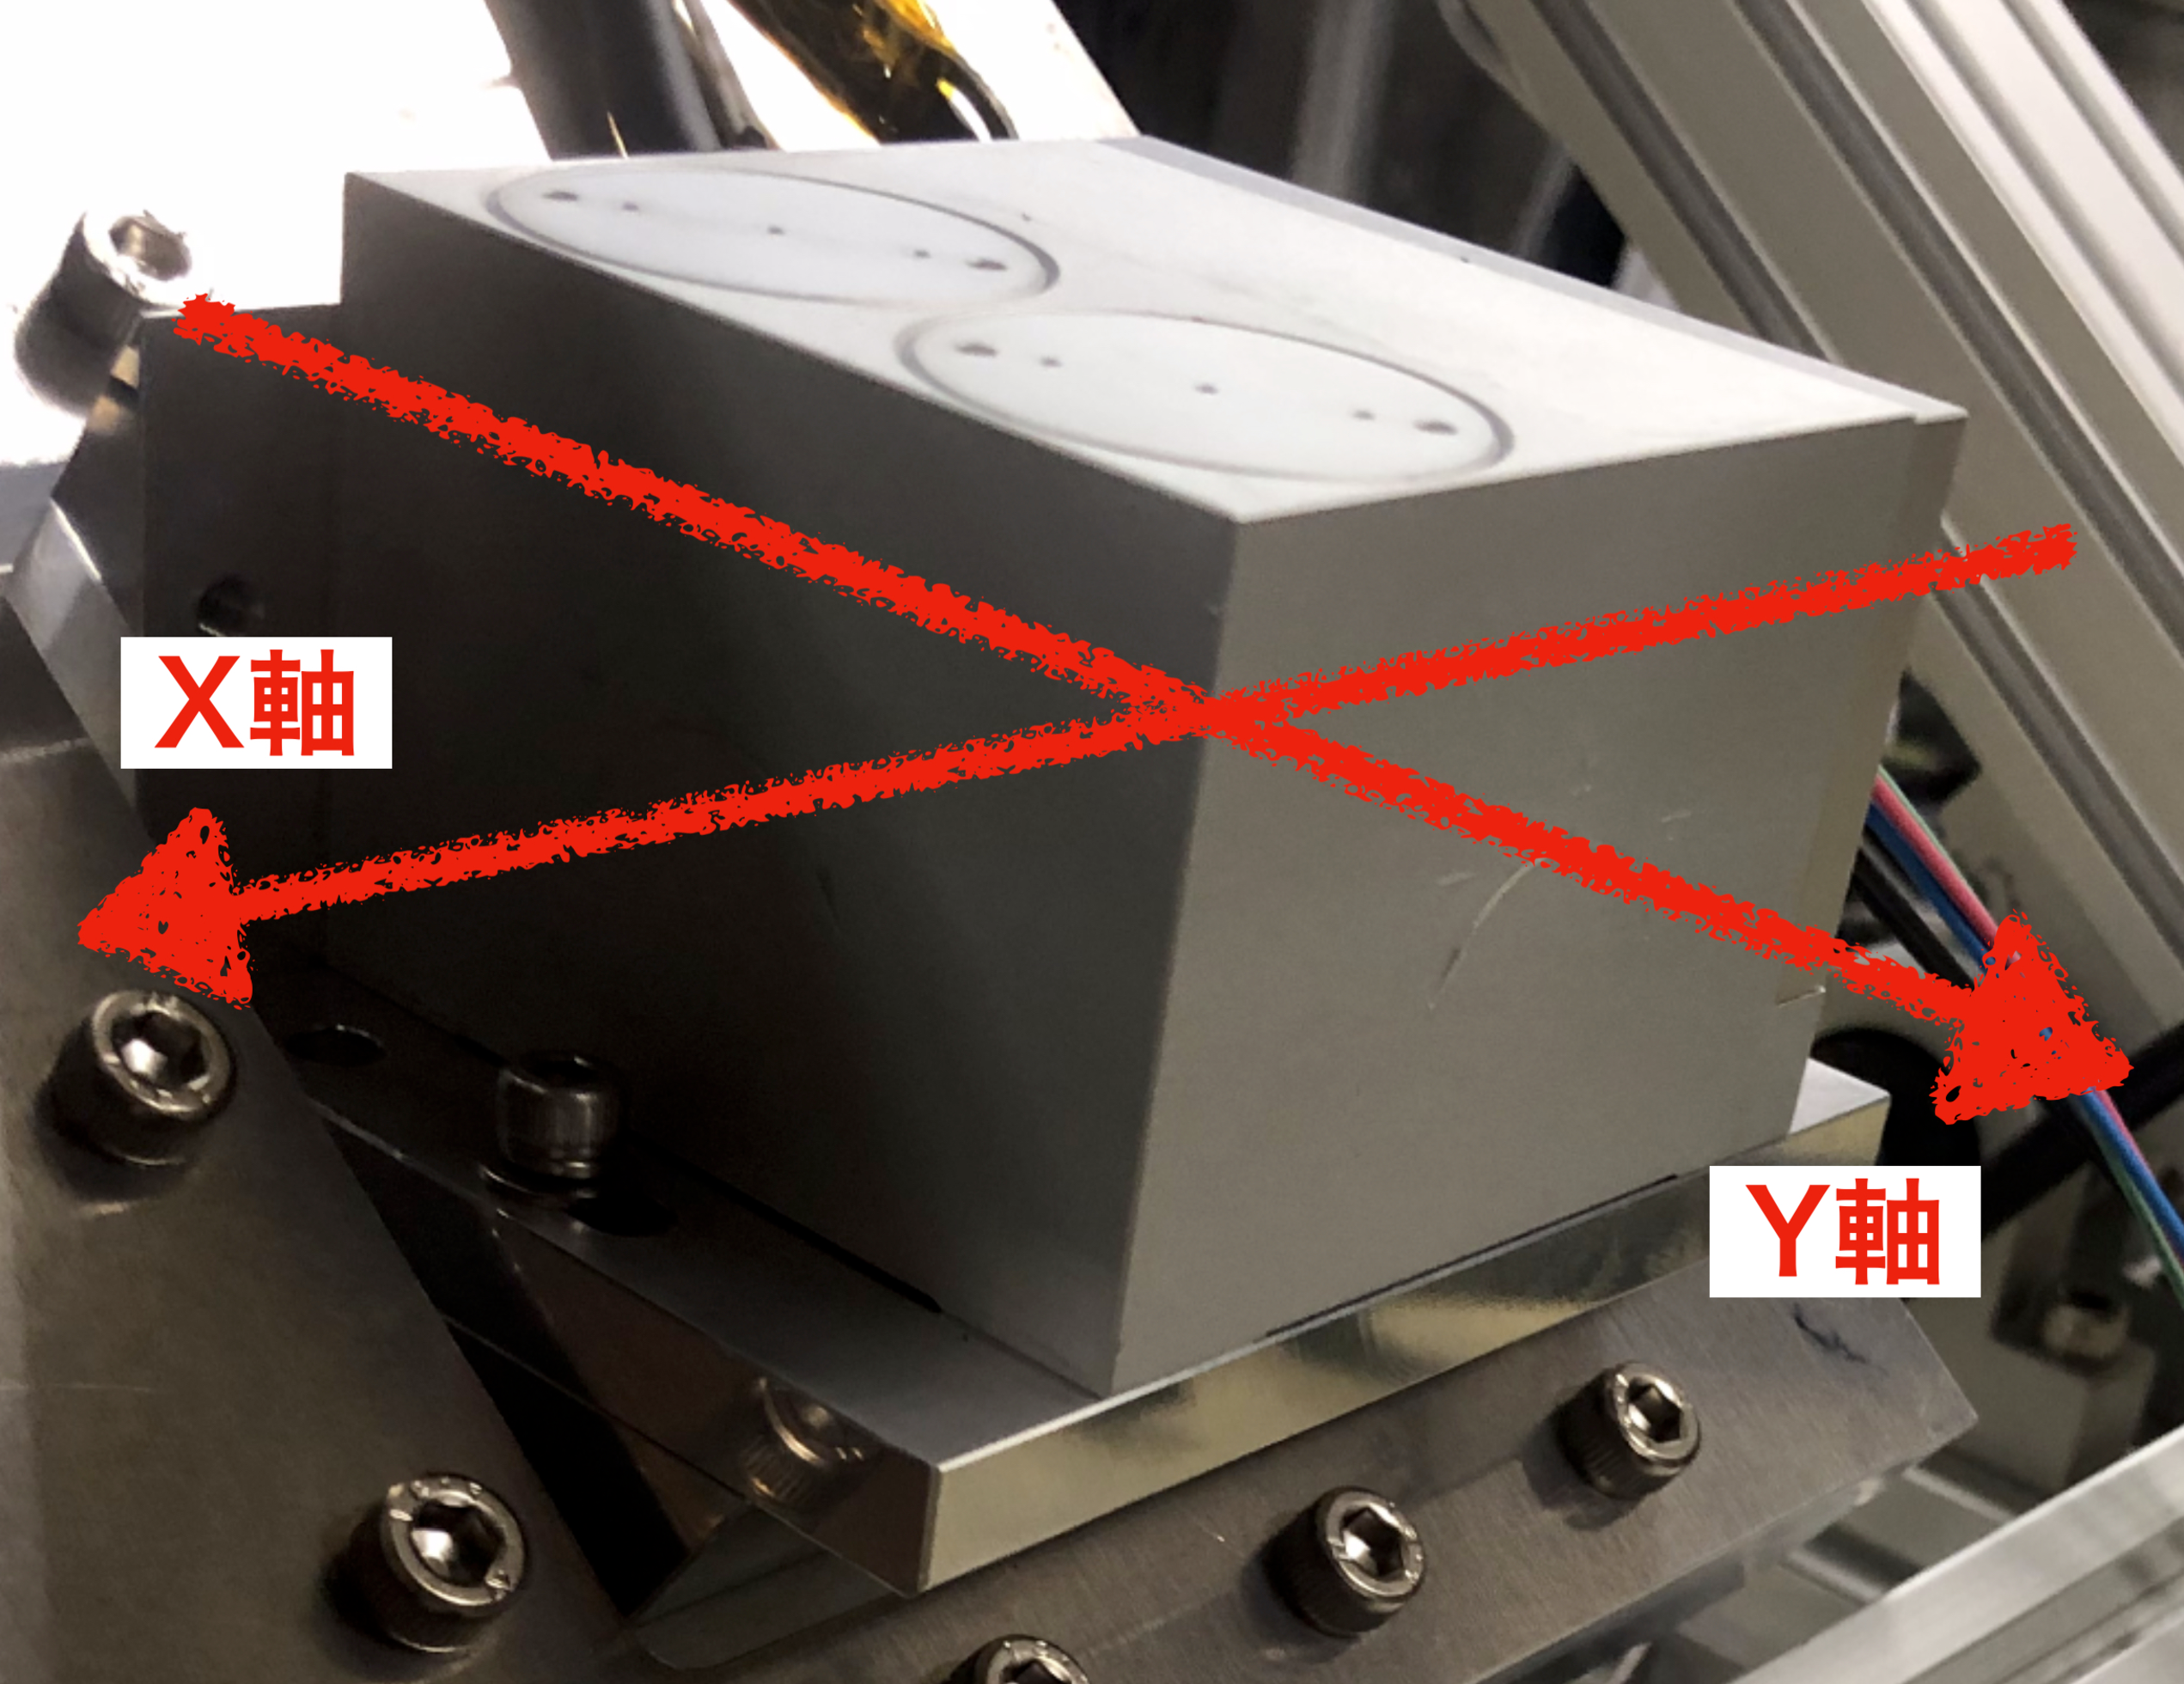
\includegraphics[width=0.65\textwidth]{tiltsensor/tiltsensor_overview.pdf}
    \figcaption{重力参照計 Sherborne Sensors 社 DSIC-2051-60 の外観}
    \label{fig:tiltsensor_DSIC-2051-60}
\end{figure}
% \begin{figure}
%     \centering
%     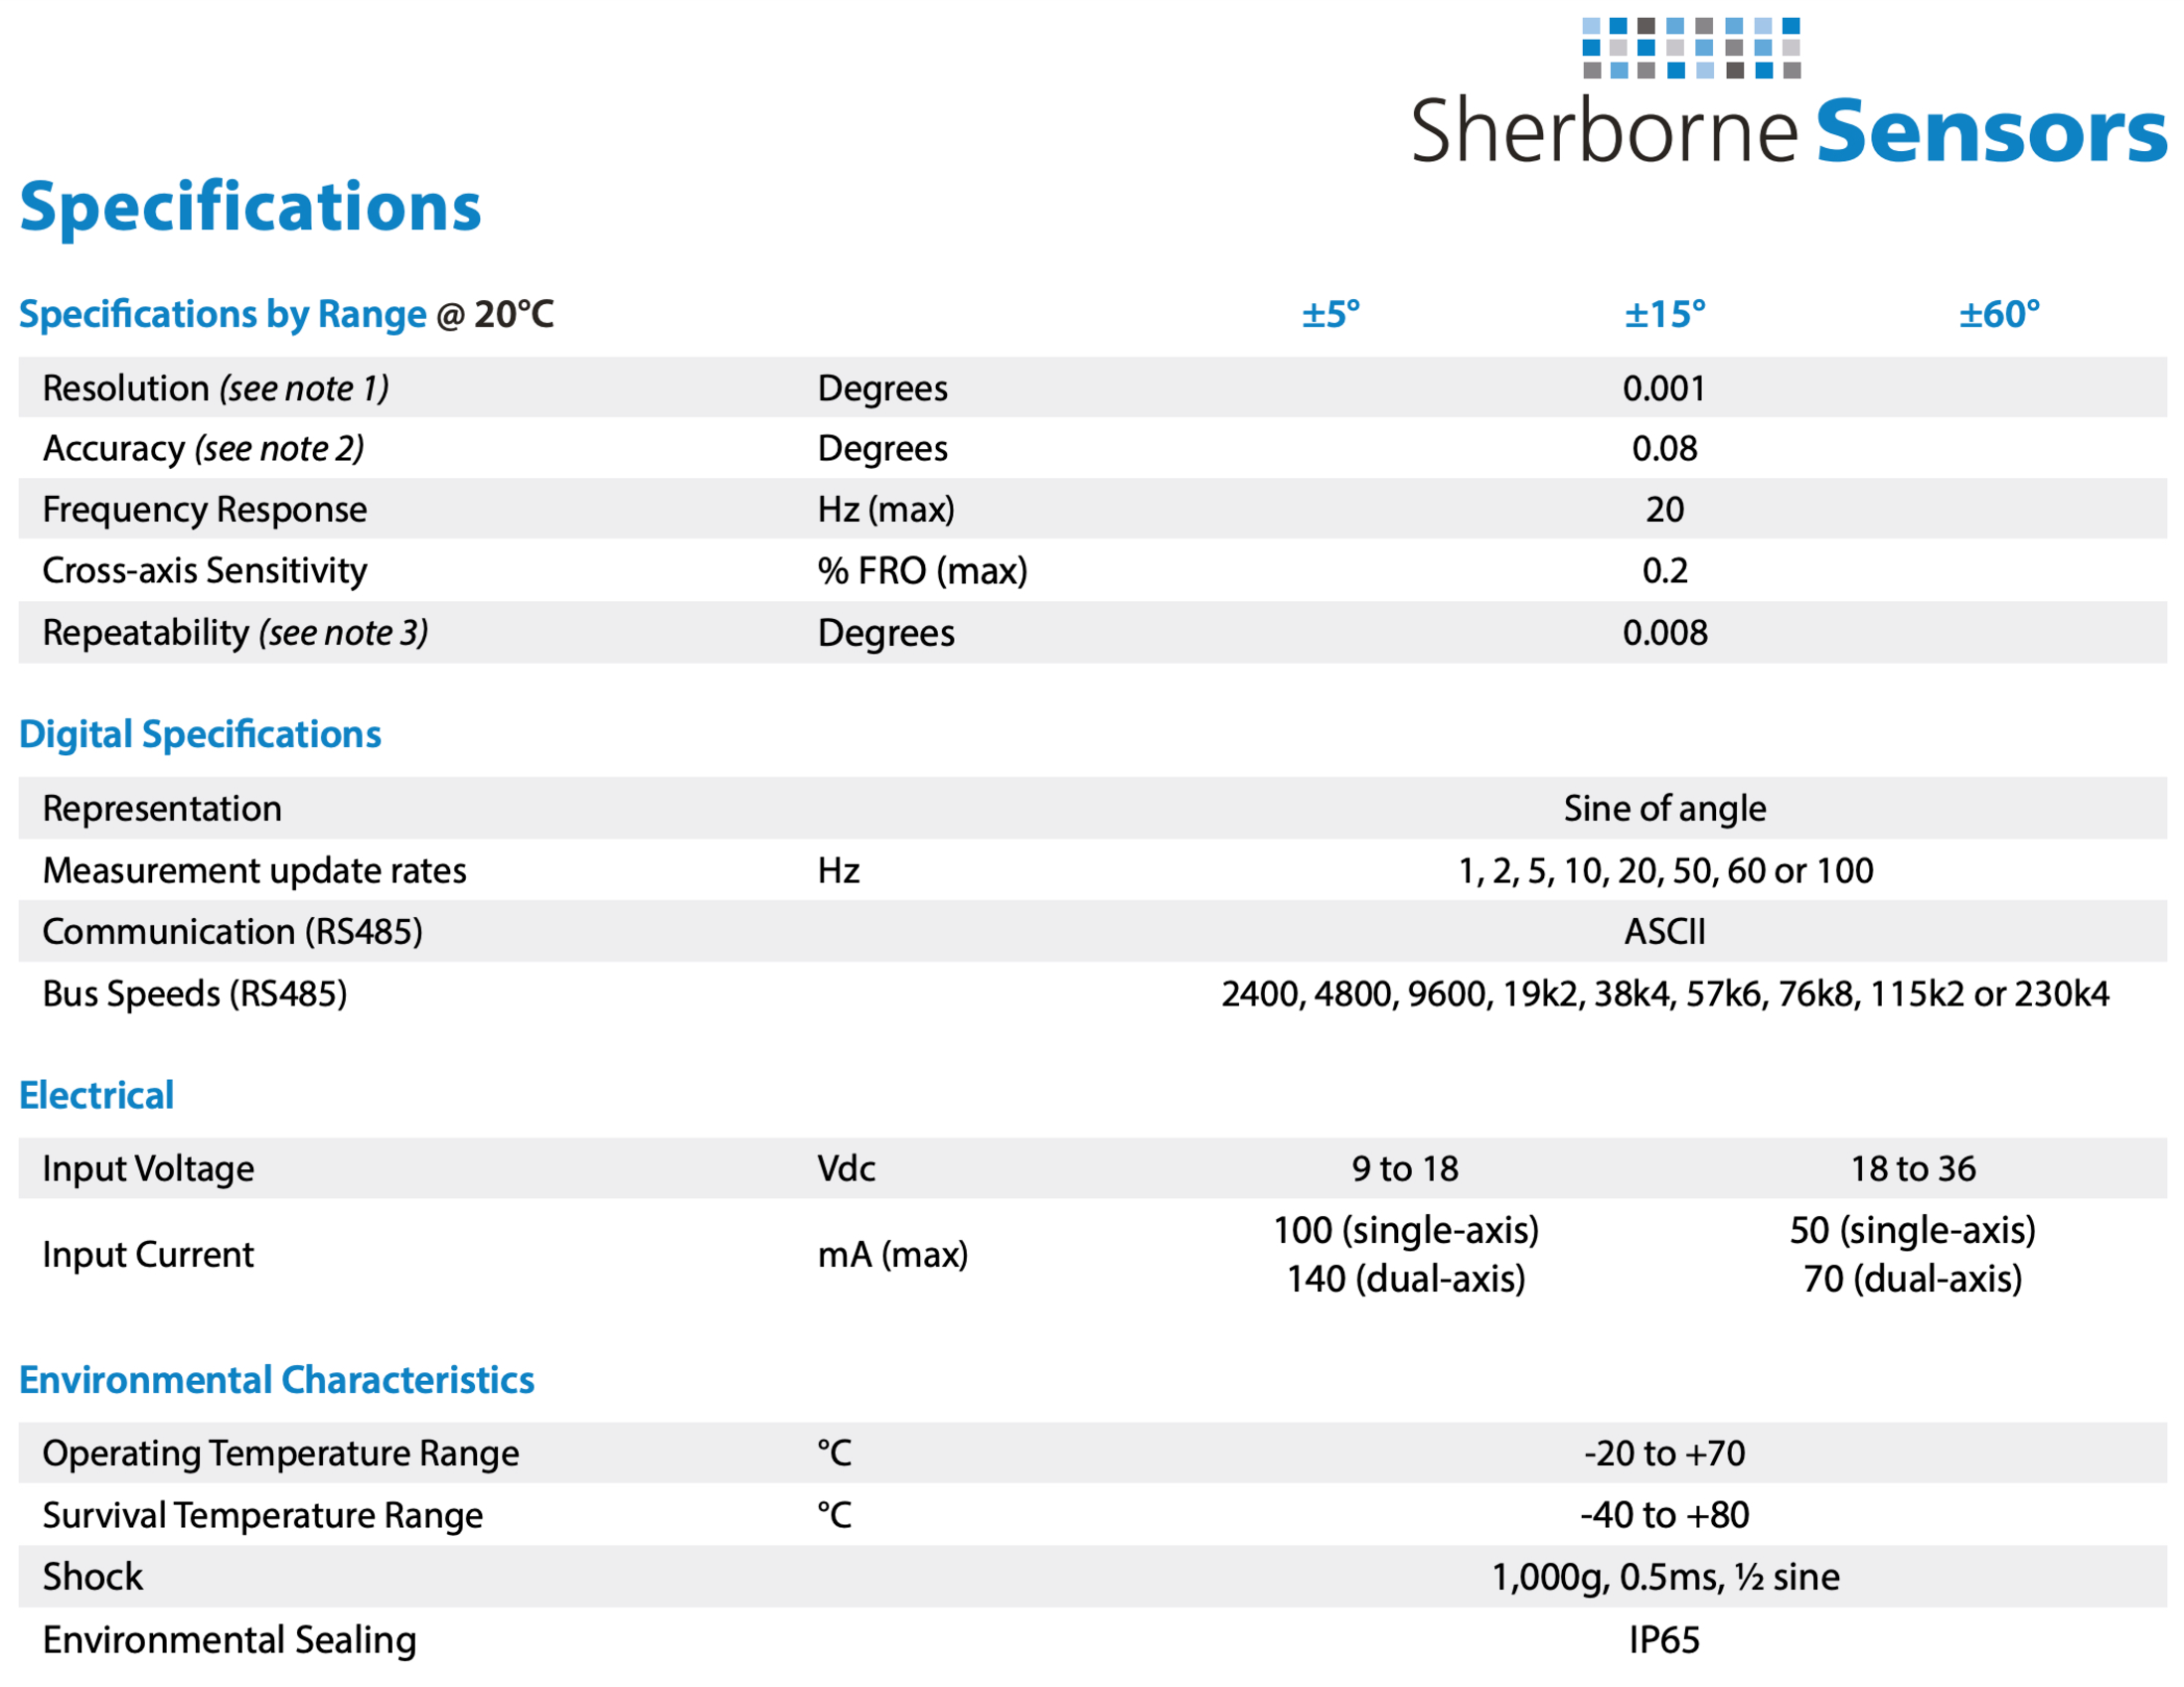
\includegraphics[width=0.5\textwidth]{tiltsensor/sherborne_spec.pdf}
%     \caption{重力参照計 Sherborne Sensors 社 DSIC-2051-60 の仕様}
%     \label{fig:tiltsensor_spec}
% \end{figure}

% \section{電源の入れ直しによるオフセット変動の評価}
% \subsection{評価系}
% 本評価における測定系を図\ref{}に示す。
%水平な机の上に重力参照計を設置した上で、以下の2つの測定を行った。
%\begin{itemize}
%    \item 電源を入れた直後から、10分間データを取得
%    \item 電源を入れた直後100秒待ち、その後30秒間データを取得
%\end{itemize}
%\subsection{測定結果}
%図\ref{}に電源を入れた直後に10分間測定した結果を示す。
\section{長期間測定における出力の安定性の評価}
\subsection{評価手法}
図\ref{fig:timedrift_evaluation_system}に評価系を示す。
重力参照計を鉄製の厚み $\SI{10}{mm}$ のプレートの上に設置した。
このプレートには3つのアジャスターが取り付けられており、これを回すことでプレートの傾きを調整できる。
プレートには新潟精機製の気泡管水準器 FLW-200002 を2つ互いに垂直になるように設置し、これを参照して
プレート全体が水平になるようにアジャスターで調整した。
この時の水平度の精度は気泡管水準器の精度によって決まり、 $< 0.01\tcdegree$ である。
この系を長期間保持したまま、重力参照計の出力する温度と角度を測定した。
測定期間は2024年3月8日から4月9日までの32日間である。
また、測定系はカメラによって1時間ごとに撮影され、気泡管水準器の気泡の位置が変化していないかを確認した。
その結果、気泡の位置に変動はあったものの水平度が $< 0.01\tcdegree$ に収まっていることが確認できた。
\begin{figure}[H]
    \centering
    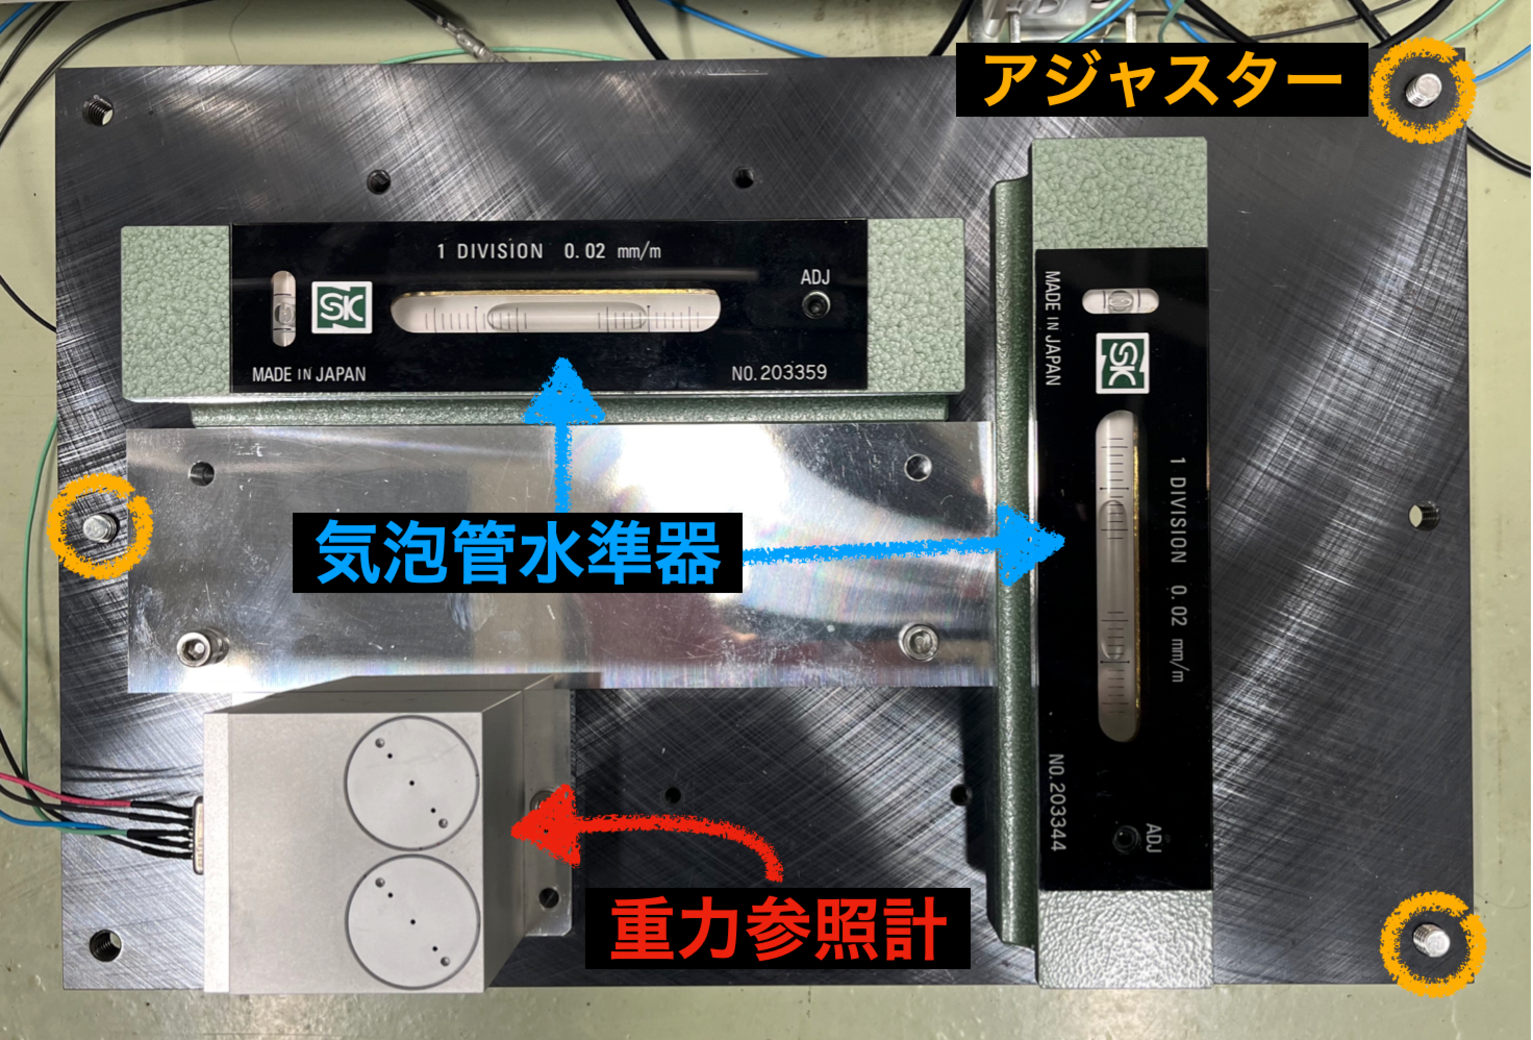
\includegraphics[width=0.7\textwidth]{tiltsensor/timedrift_evaluation_system.pdf}
    \caption{長期間測定における重力参照計の評価系}
    \label{fig:timedrift_evaluation_system}
\end{figure}

\subsection{評価結果とその考察}
図\ref{fig:timedrift_Xaxis}および\ref{fig:timedrift_Yaxis}に測定された温度と角度を日毎に平均をとった結果を示す。
誤差として、各日のデータ群の標準偏差を示している。
$X$ 軸については、日毎に平均された出力角度の平均が $-0.0598\tcdegree$ となり、その標準偏差は $0.0028\tcdegree$ であった。
この結果から、時間変化による出力角度の変化の精度を $\delta\theta_{X,\mathrm{time}} = 0.003\tcdegree$ であると結論づける。
$Y$ 軸については、日毎に平均された出力角度の平均が $-0.012\tcdegree$ となり、その標準偏差は $0.034\tcdegree$ であった。
この結果から、時間変化による出力角度の変化の精度を $\delta\theta_{Y,\mathrm{time}} = 0.034\tcdegree$ であると結論づける。
表\ref{tab:timedrift_result}にこれらの結果をまとめる。
$Y$ 軸の結果は $X$ 軸の結果に比べ非常に大きな値となっている。
図\ref{fig:timedrift_Yaxis}(\subref{fig:timedrift_tempY})と
図\ref{fig:timedrift_Yaxis}(\subref{fig:timedrift_angleY})を見比べると
温度の変動に伴って出力角度が大きく変化しており、この精度の違いは温度変動による出力角度の変化が $X$ 軸と $Y$ 軸で異なることが原因であると考えられる。
次節の温度変動による出力の変化の評価にてこれを検証する。
\begin{figure}[H]
    \begin{minipage}[b]{0.45\columnwidth}
        \centering
        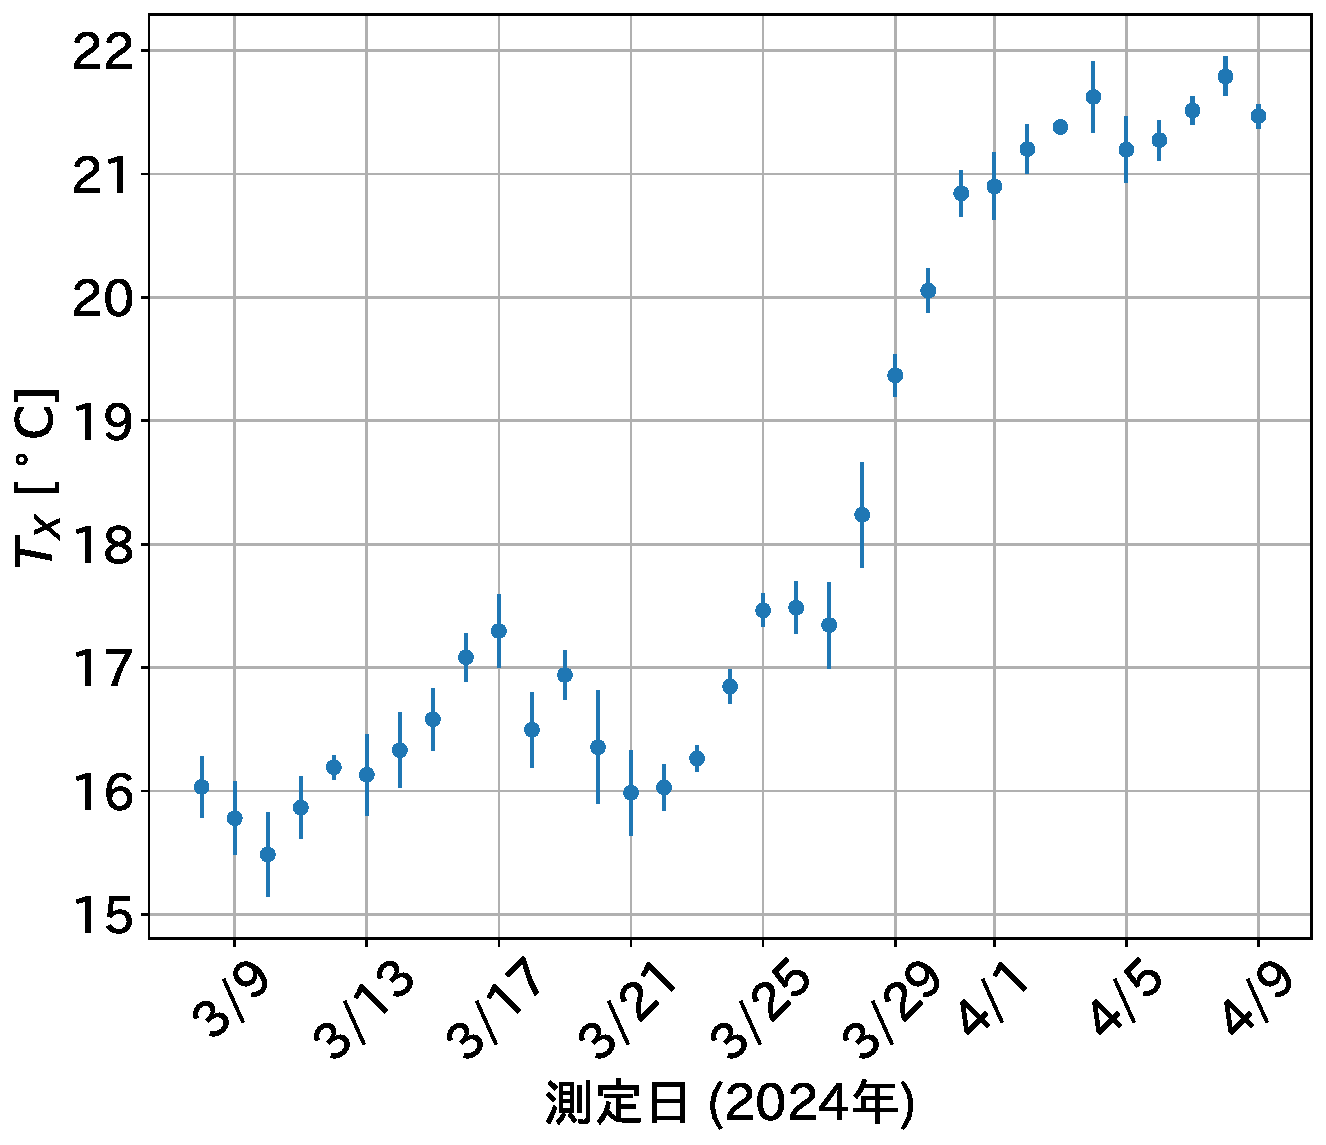
\includegraphics[width=1.0\columnwidth]{tiltsensor/timedrift_tempX_daily.pdf}
        \subcaption{}
        \label{fig:timedrift_tempX}
    \end{minipage}
    \hspace{2mm}
    \begin{minipage}[b]{0.527\columnwidth}
        \centering
        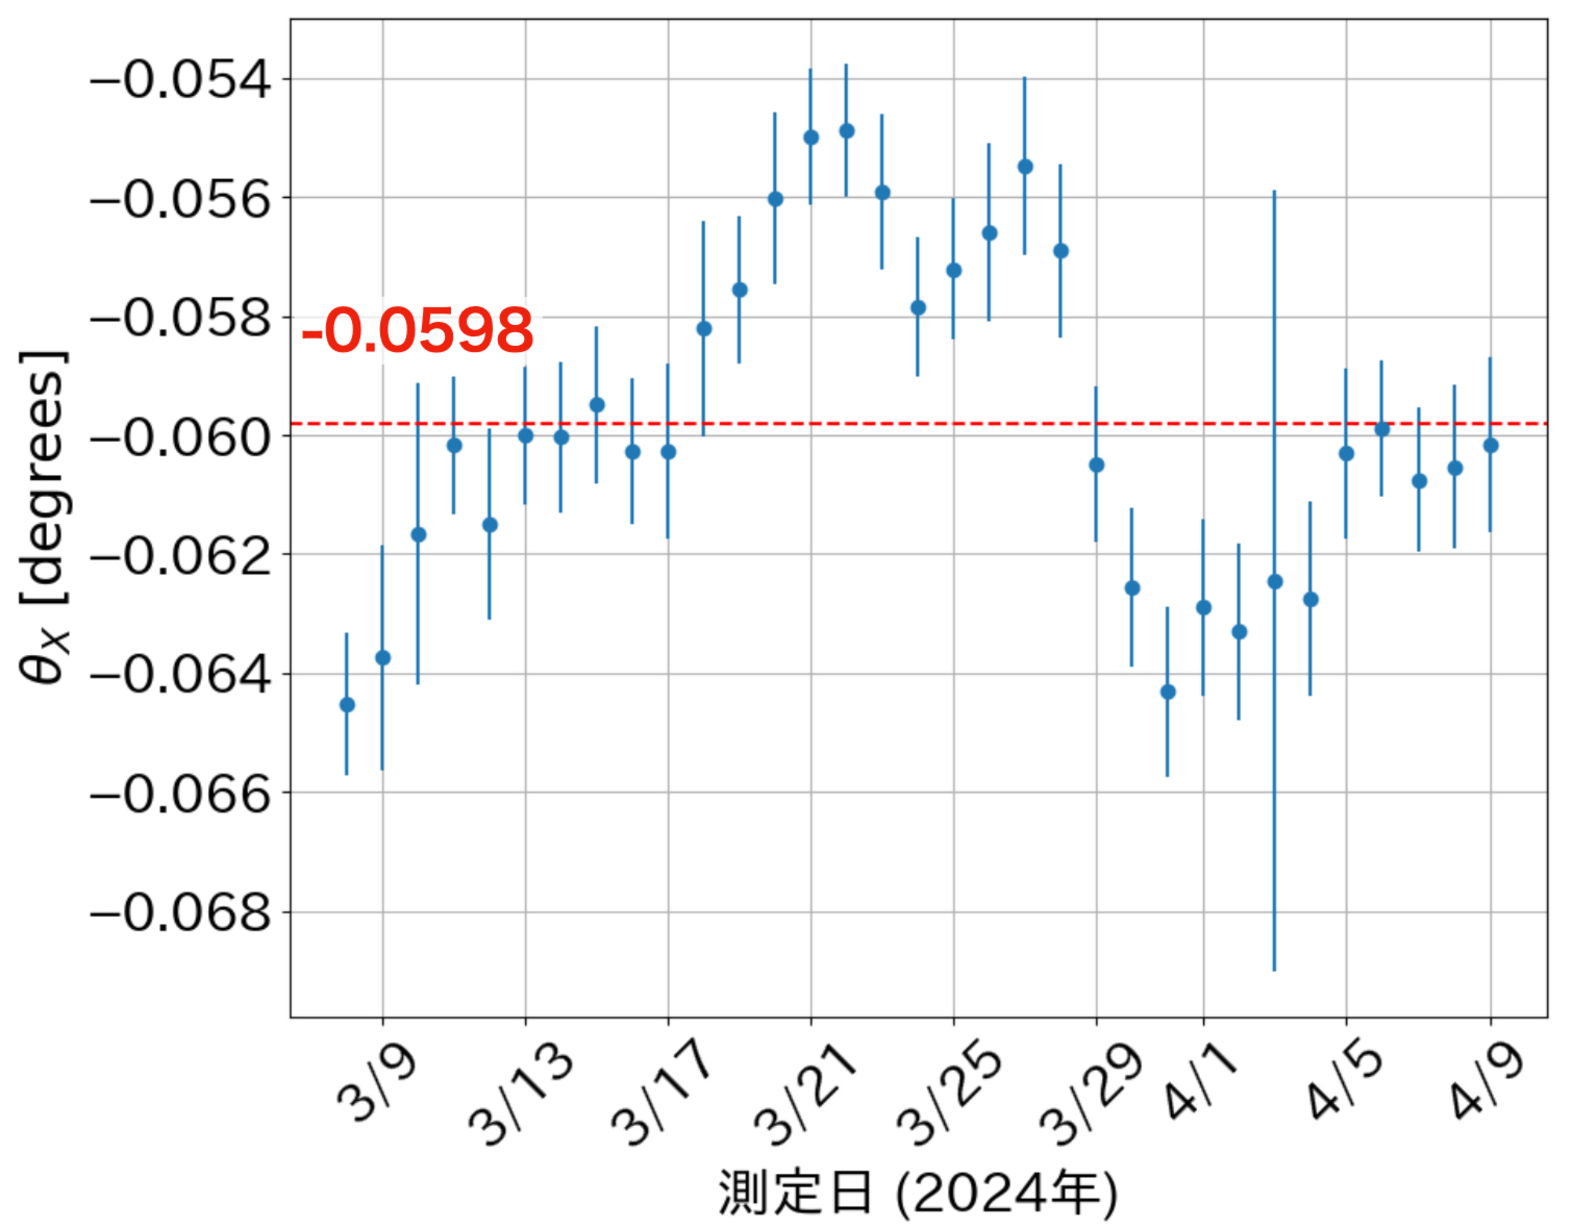
\includegraphics[width=0.95\columnwidth]{tiltsensor/timedrift_angleX_daily.pdf}
        \subcaption{}
        \label{fig:timedrift_angleX}
    \end{minipage}
    \caption{日毎に平均化された1ヶ月間の $X$ 軸の温度と角度の変化。
             (\subref{fig:timedrift_tempX}) $X$ 軸の出力温度 $T_{X}$ の変化。
             (\subref{fig:timedrift_angleX}) $X$ 軸の出力角度 $\theta_{X}$ の変化。}
    \label{fig:timedrift_Xaxis}
\end{figure}
\begin{figure}[H]
    \begin{minipage}[b]{0.45\columnwidth}
        \centering
        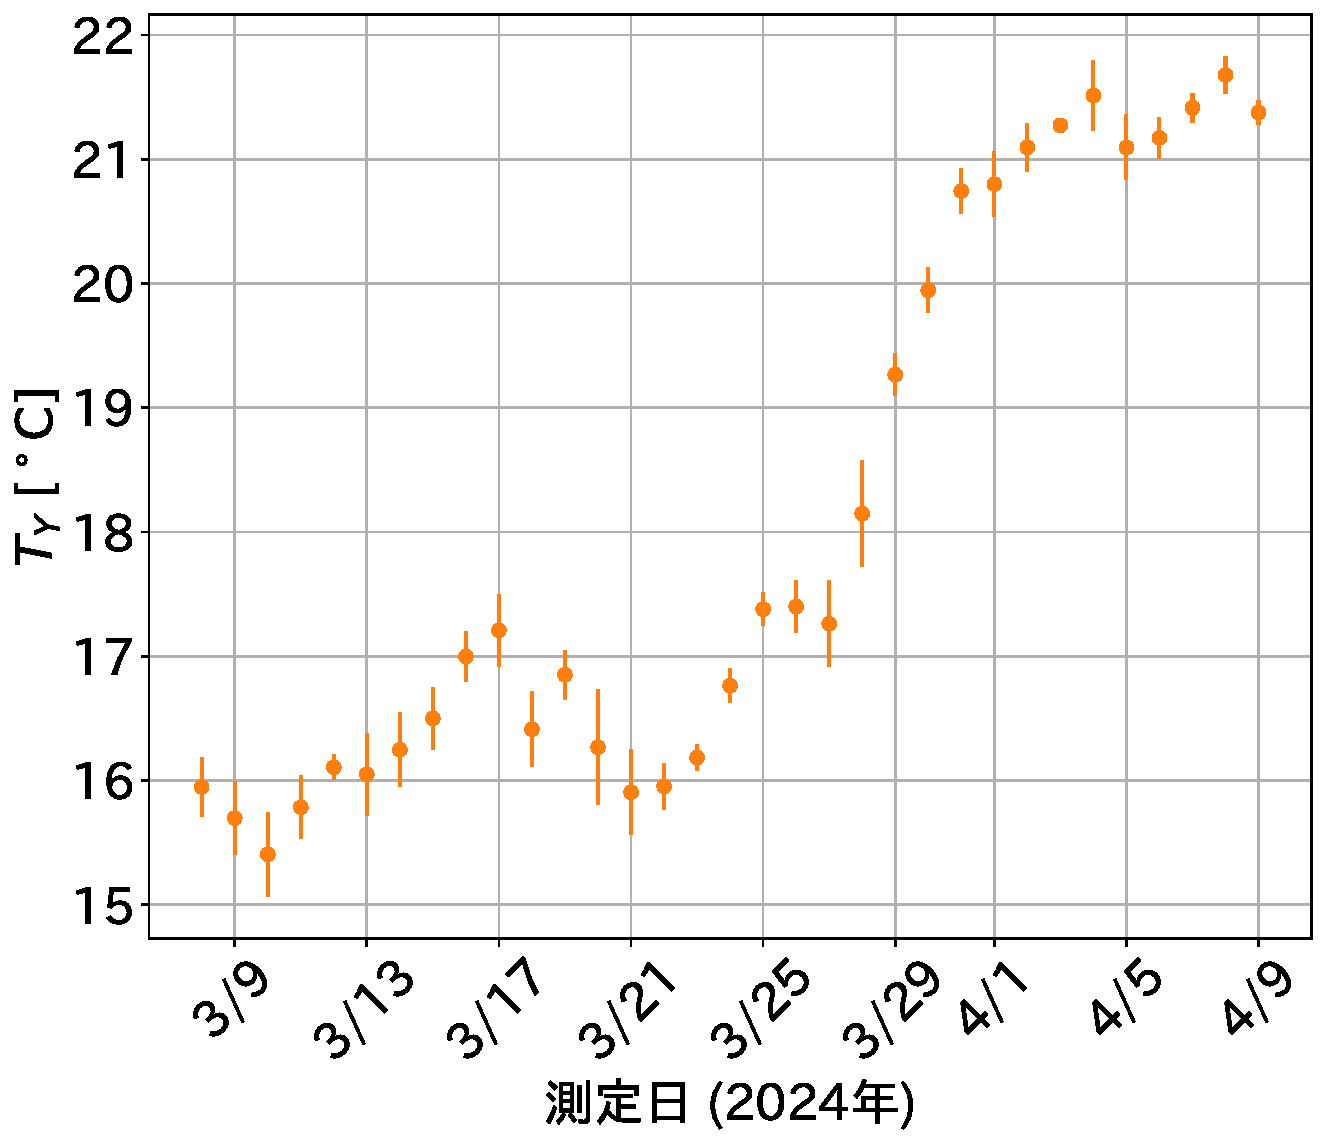
\includegraphics[width=1.0\columnwidth]{tiltsensor/timedrift_tempY_daily.pdf}
        \subcaption{}
        \label{fig:timedrift_tempY}
    \end{minipage}
    \hspace{2mm}
    \begin{minipage}[b]{0.49\columnwidth}
        \centering
        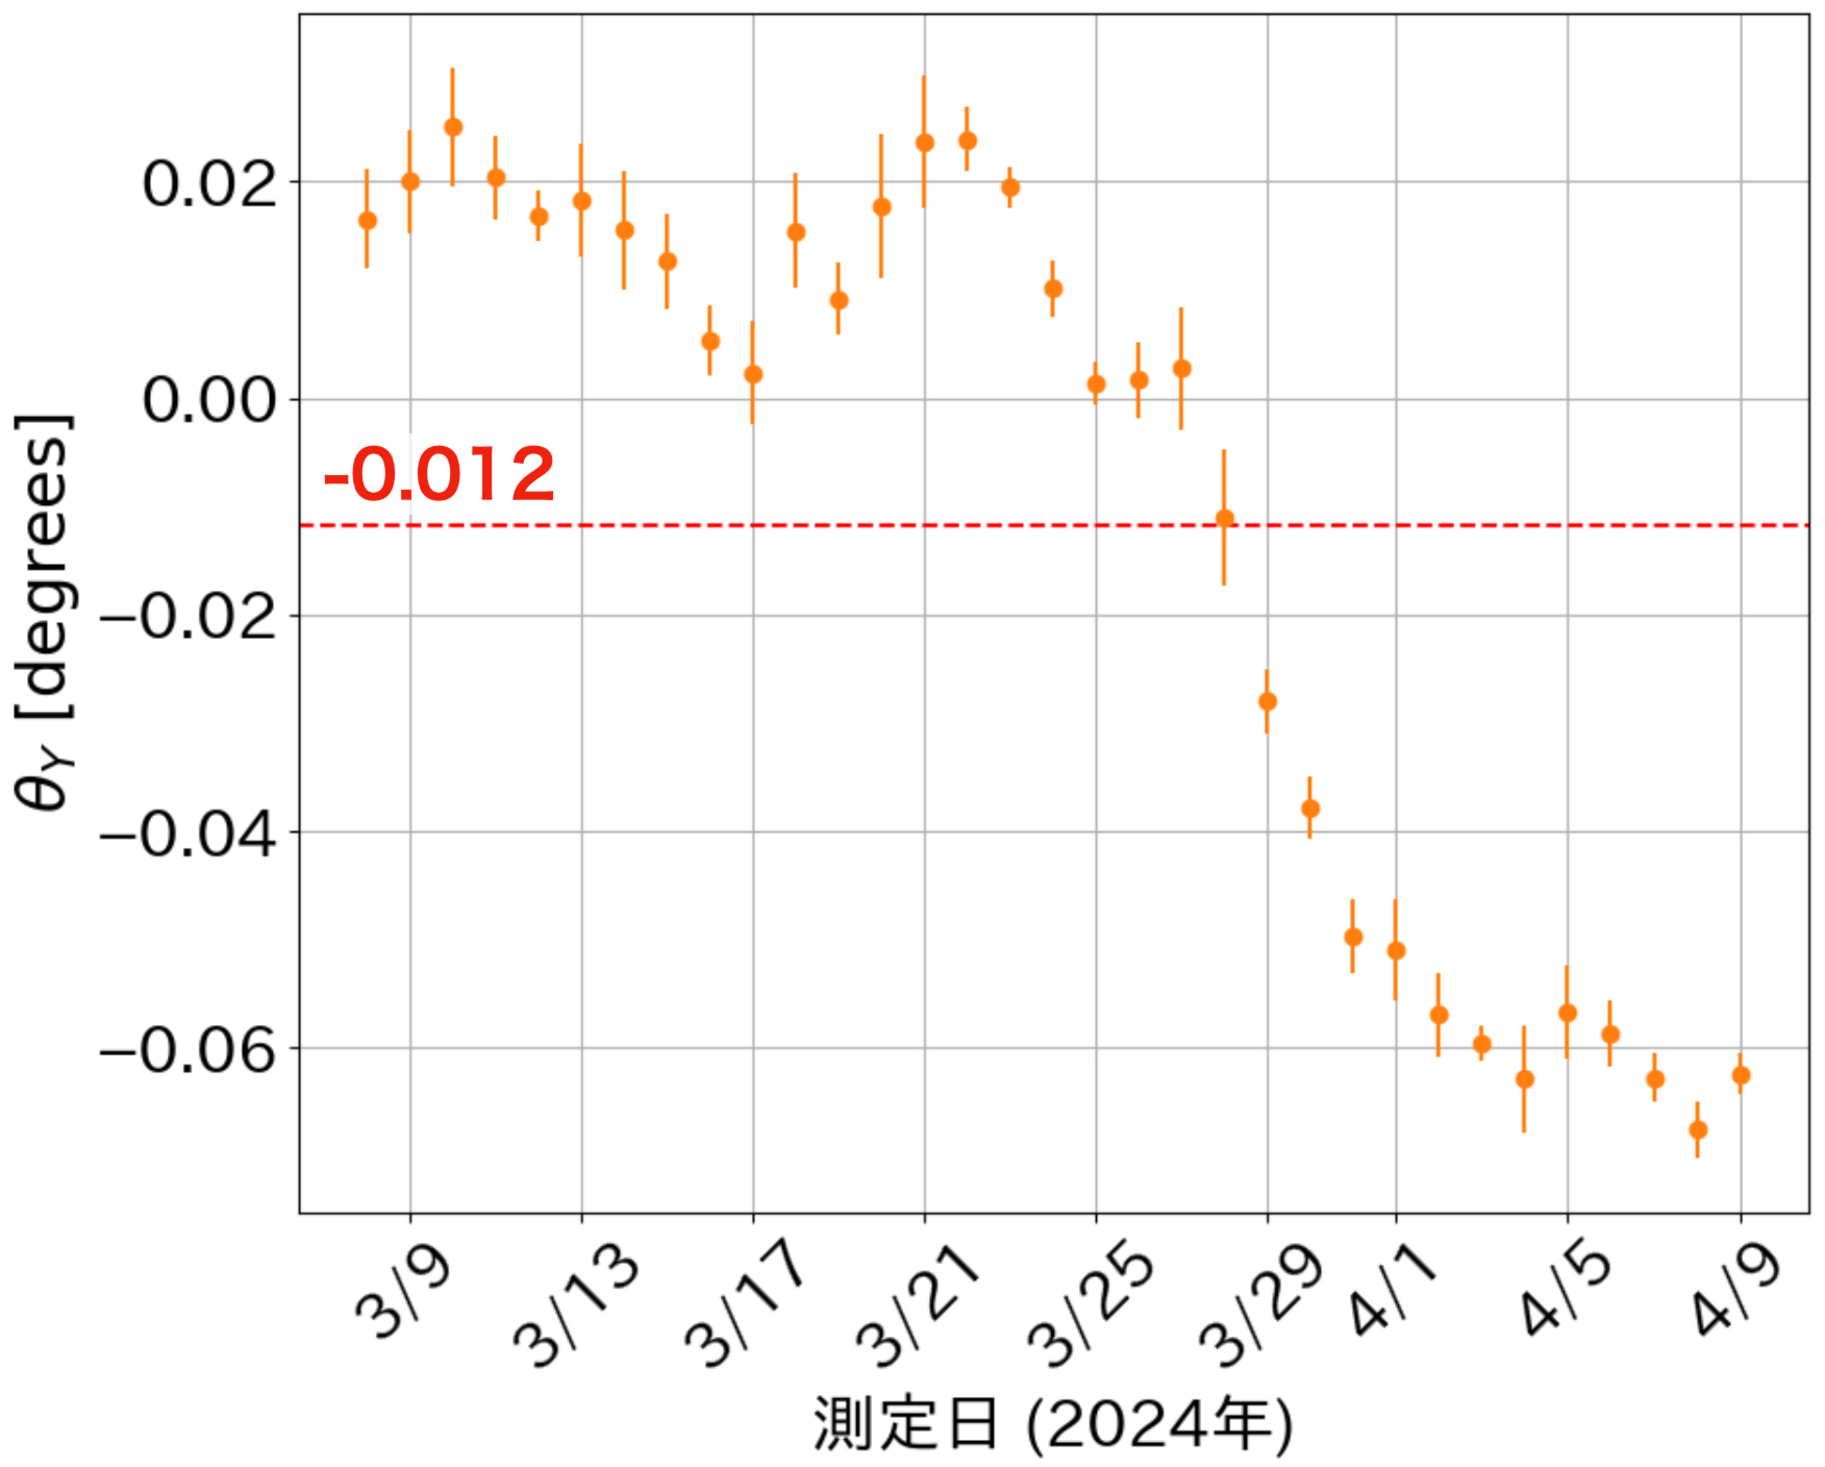
\includegraphics[width=0.985\columnwidth]{tiltsensor/timedrift_angleY_daily.pdf}
        \subcaption{}
        \label{fig:timedrift_angleY}
    \end{minipage}
    \caption{日毎に平均化された1ヶ月間の $Y$ 軸の温度と角度の変化。
    (\subref{fig:timedrift_tempY}) $Y$ 軸の出力温度 $T_{Y}$ の変化。
    (\subref{fig:timedrift_angleY}) $Y$ 軸の出力角度 $\theta_{Y}$ の変化。}
    \label{fig:timedrift_Yaxis}
\end{figure}
\begin{table}[H]
    \centering
    \caption{長期間測定における重力参照計の出力の安定性の評価結果}
    \begin{tabular}{cccc} \hline
        & 平均 & 標準偏差 & 精度 \\ \hline\hline
        $X$ 軸 & $-0.0598\tcdegree$ & $0.0028\tcdegree$ & $0.003\tcdegree$ \\ \hline
        $Y$ 軸 & $-0.012\tcdegree$ & $0.034\tcdegree$ & $0.034\tcdegree$ \\ \hline
    \end{tabular}
    \label{tab:timedrift_result}
\end{table}

\section{温度変動による出力の変化の評価}
\subsection{評価手法}
図\ref{fig:temp_evaluation_system}に評価系を示す。
重力参照計をアルミニウム製の厚み $\SI{30}{mm}$ のプレートの上に設置した。
長期間測定における出力の変化の評価の際と同様に、
このプレートには3つのアジャスターが取り付けられており、これを回すことでプレートの傾きを調整できる。
プレートには新潟精機製の気泡管水準器 FLW-200002 を2つ互いに垂直になるように設置し、これを参照して
プレート全体が水平になるようにアジャスターで調整した。
この時の水平度の精度は気泡管水準器の精度によって決まり、 $< 0.01\tcdegree$ である。
また、プレート上にはUSB温度計を設置し、周囲の空気の温度を測定した。
以上の測定系を恒温槽\footnote{恒温槽は京都市産業技術研究所より拝借した。}に入れ、温度を変化させたときの出力を測定した。

図\ref{fig:bath_temp_usb}にUSB温度計を用いて測定した恒温槽内の温度 $T_{\mathrm{USB}}$ の変化の様子を示す。
$\SI{20}{\degreeCelsius}$ から $\SI{-20}{\degreeCelsius}$ まで冷却したのち、再び $\SI{20}{\degreeCelsius}$ まで昇温し、出力の変化を測定した。
各温度 $\SI{10}{\tcdegree}$ 刻みで$\SI{3}{時間}$ ほどかけて変化させ、温度が安定している状態が生まれるようにした。
測定中にはWebカメラを用いて10分ごとに撮影し、気泡管水準器の気泡の位置が変化していないかを確認した。
例として、図\ref{fig:evaluation_bath_camera}(\subref{fig:camera_12degC})に
$T_{\mathrm{USB}} \sim \SI{12}{\degreeCelsius}$ で撮影された写真を、
図\ref{fig:evaluation_bath_camera}(\subref{fig:camera_m18degC})に
$T_{\mathrm{USB}} \sim \SI{-18}{\degreeCelsius}$ で撮影された写真を示す。
全ての写真を確認したところ、気泡の位置に変動はあったものの水平度が $< 0.01\tcdegree$ に収まっていることが確認できた。

\begin{figure}[H]
    \centering
    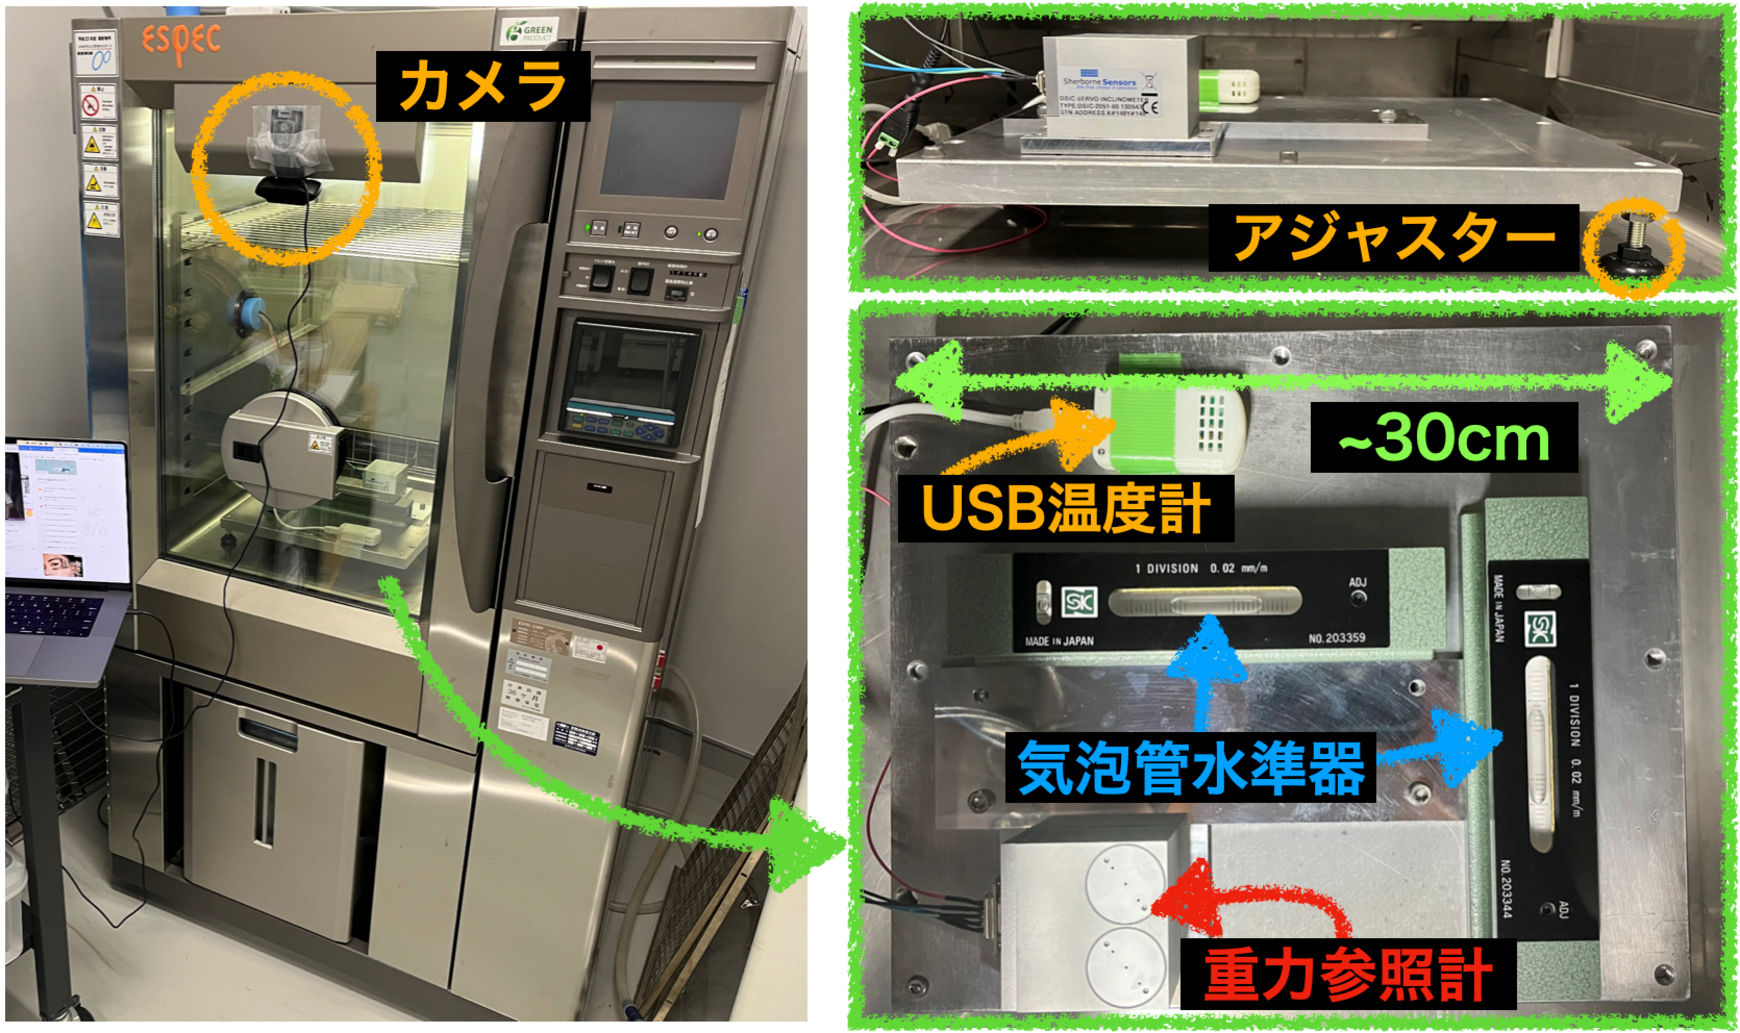
\includegraphics[width=1.0\textwidth]{tiltsensor/temp_evaluation_system.pdf}
    \figcaption{恒温槽を用いた重力参照計の温度変化評価系}
    \label{fig:temp_evaluation_system}
\end{figure}
\begin{figure}[H]
    \centering
    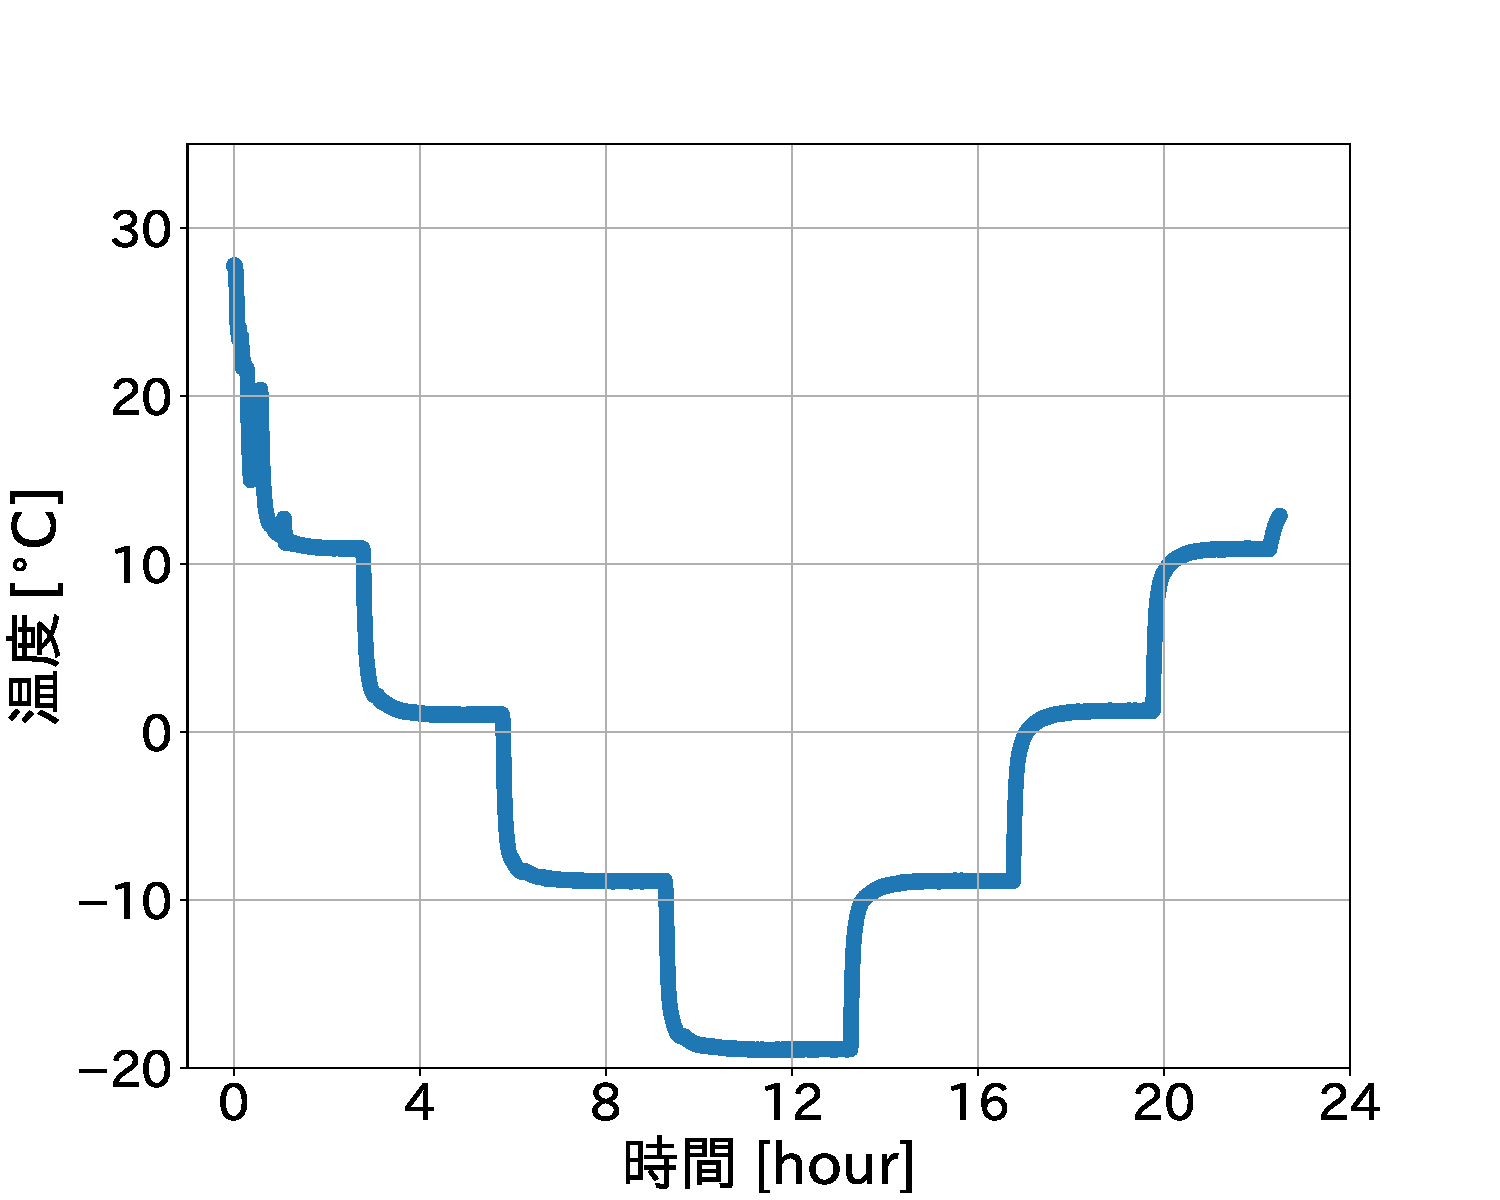
\includegraphics[width=0.8\textwidth]{tiltsensor/bath_temp_usb.pdf}
    \figcaption{恒温槽の温度変化}
    \label{fig:bath_temp_usb}
\end{figure}
\begin{figure}[tbp]
    \begin{minipage}[b]{0.45\columnwidth}
        \centering
        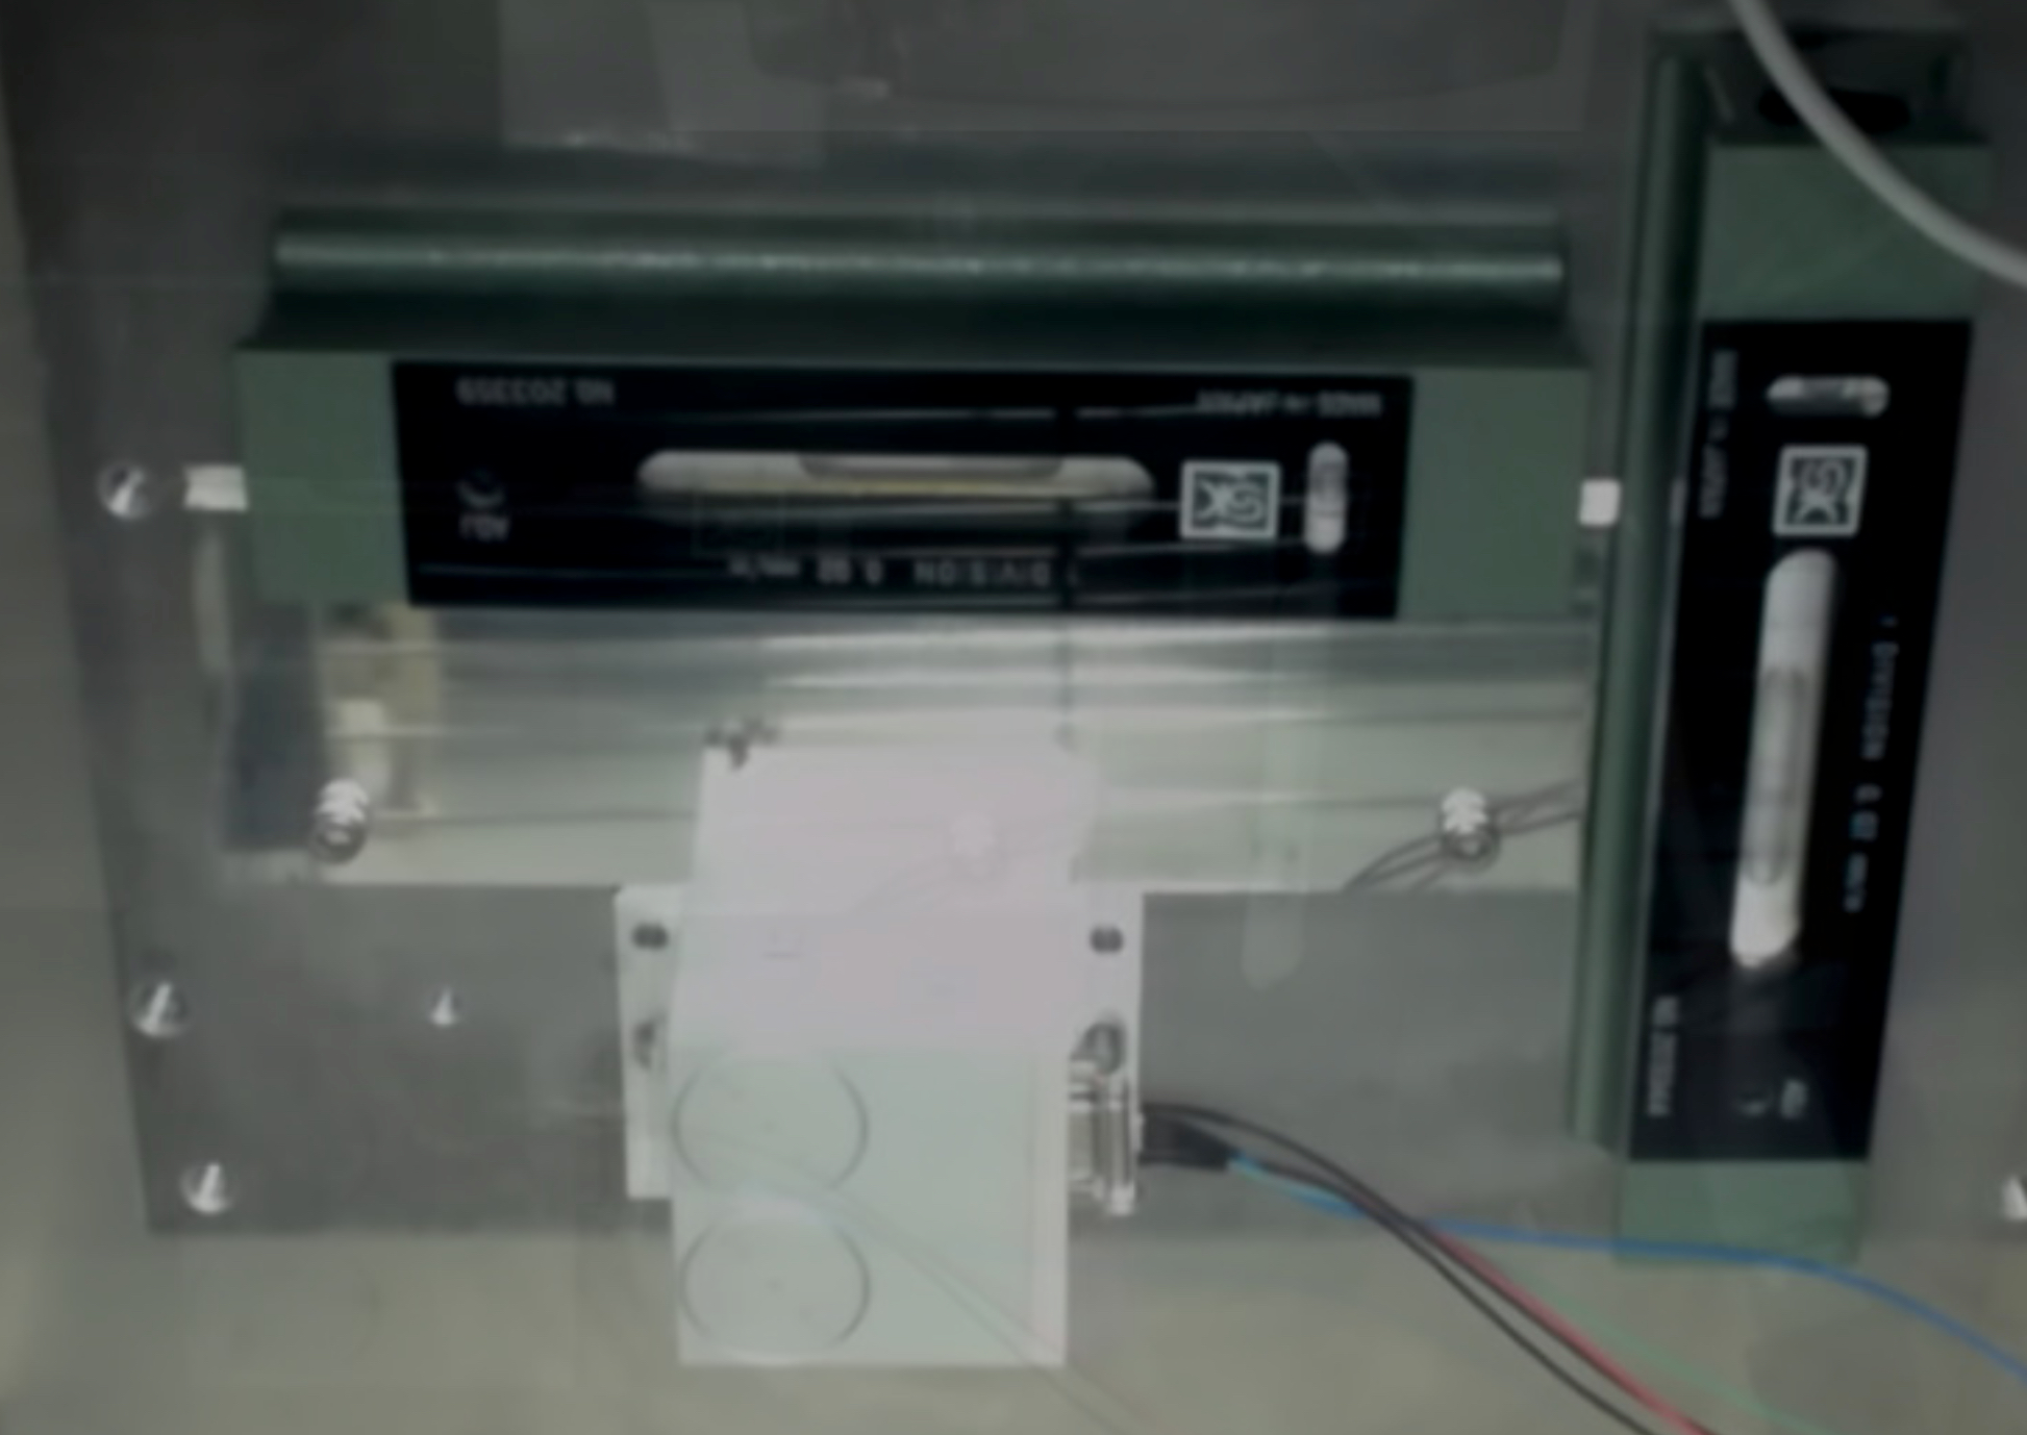
\includegraphics[width=1.0\columnwidth]{tiltsensor/camera_12degC.pdf}
        \subcaption{}
        \label{fig:camera_12degC}
    \end{minipage}
    \hspace{0.06\columnwidth}
    \begin{minipage}[b]{0.45\columnwidth}
        \centering
        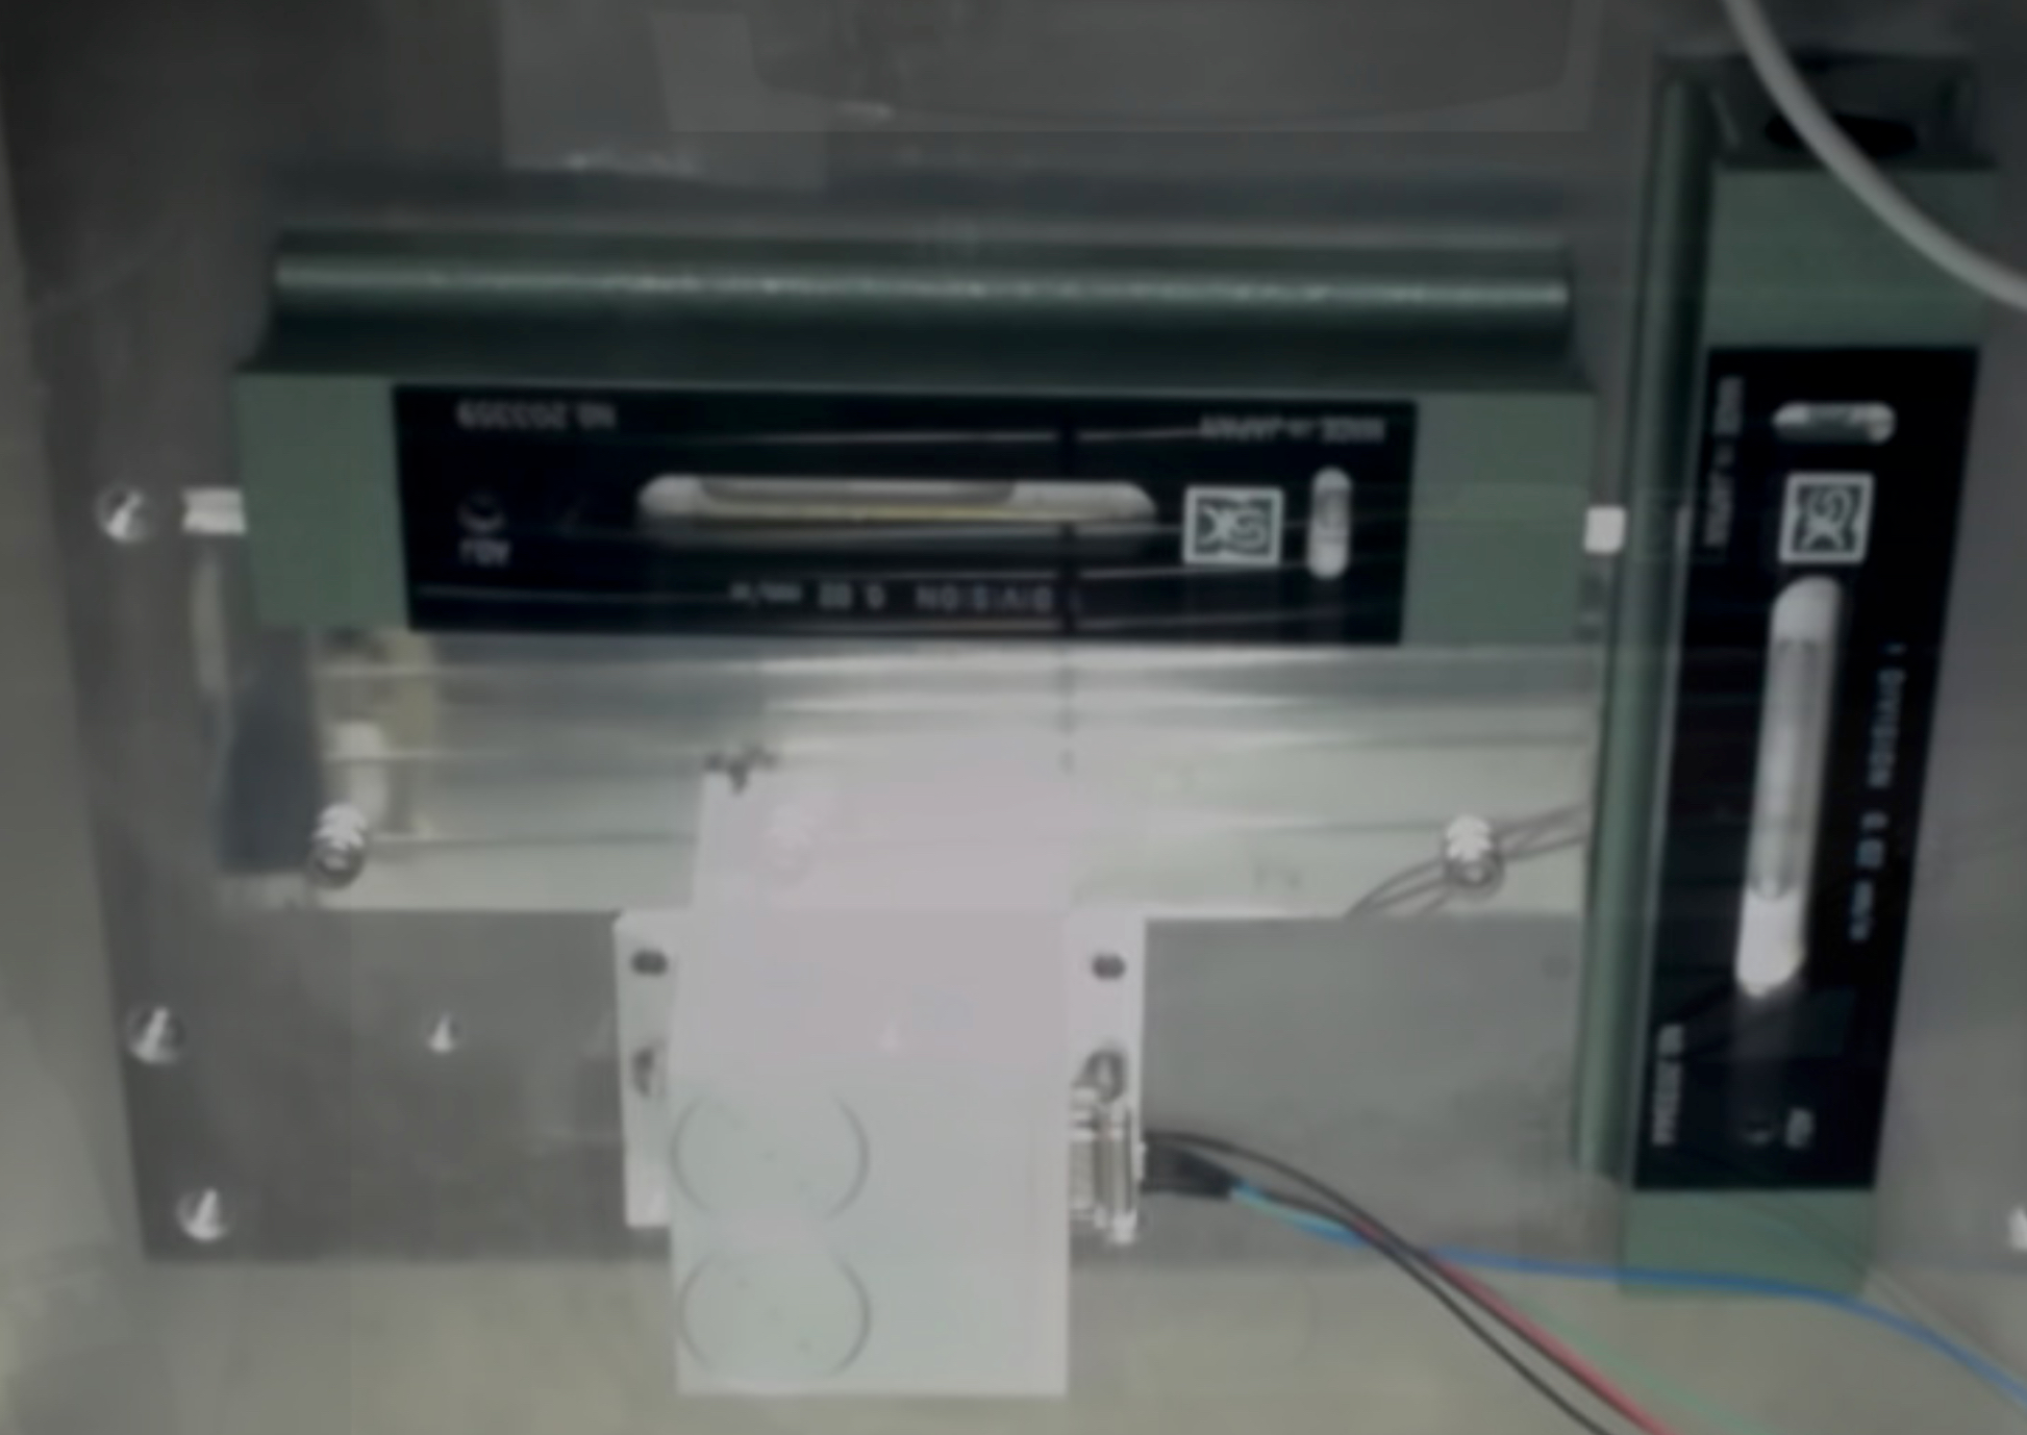
\includegraphics[width=1.0\columnwidth]{tiltsensor/camera_m18degC.pdf}
        \subcaption{}
        \label{fig:camera_m18degC}
    \end{minipage}
    \caption{Webカメラを用いて撮影された恒温槽内の様子。
             (\subref{fig:camera_12degC}) $T_{\mathrm{USB}} \simeq \SI{12}{\degreeCelsius}$ で撮影された写真。
             (\subref{fig:camera_m18degC}) $T_{\mathrm{USB}} \simeq \SI{-18}{\degreeCelsius}$ で撮影された写真。}
    \label{fig:evaluation_bath_camera}
\end{figure}
\subsection{評価結果とその考察}
観測サイトでの気温変動は十分ゆっくりであるか、較正の時間帯を選ぶことで急激な温度変化を避けることができるため、
恒温槽の温度が安定し、評価計全体と熱平衡であるような状態のデータを用いて評価を行う。
図\ref{fig:evaluation_bath_Xaxis}に重力参照計の $X$ 軸が出力する温度 $T_{X}$ と、その温度が安定的になったときの出力角度 $\theta_{X}$ の変化を、
図\ref{fig:evaluation_bath_Yaxis}に $Y$ 軸について同様の結果を示す。
温度安定区間は、図\ref{fig:evaluation_bath_Xaxis}(\subref{fig:bath_tempX})、図\ref{fig:evaluation_bath_Yaxis}(\subref{fig:bath_tempY})において、緑色でマスクした部分である。
各温度安定時の出力角度は、それぞれ平均を取り、その標準偏差と気泡管水準器が保証する $0.01\tcdegree$ を誤差として示している。
どちらの軸に関しても、ヒステリシスを見るために冷却時と昇温時のデータを分けて示している。

$X$ 軸については、温度変化に対する出力角度の平均が $-0.023\tcdegree$ となり、その誤差の平均は $0.011\tcdegree$ であった。
この結果から、それぞれの絶対値の和を取ることで $\theta_{X}$ の精度を 
$\delta\theta_{X,\mathrm{temp}} = 0.033\tcdegree$ であると結論づける。
$Y$ 軸については、温度変化に対する出力角度の平均が $1.18\tcdegree$ となり、その誤差の平均は $0.014\tcdegree$ であった。
図\ref{fig:evaluation_bath_Yaxis}(\subref{fig:angleY_temp_dep})に示すように
温度変化に対する出力角度の変化が $2.0\tcdegree$ 以上と非常に大きく、絶対角度較正には使用できない精度であることがわかる。
これにより、前節の長期間の出力の安定性の評価において $Y$ 軸の精度が $X$ 軸に比べて悪かったことが、
温度変動による出力角度の変化によるものであると説明できる。
要求精度を満たさない結果が得られたが、この結果は公称精度 $0.08\tcdegree$ を大きく上回っており、初期不良の可能性が疑われる。
次節にて、この初期不良の可能性を検証する。
また、表\ref{tab:temp_result}にこれらの結果をまとめる。
\begin{figure}[H]
    \begin{minipage}[b]{0.45\columnwidth}
        \centering
        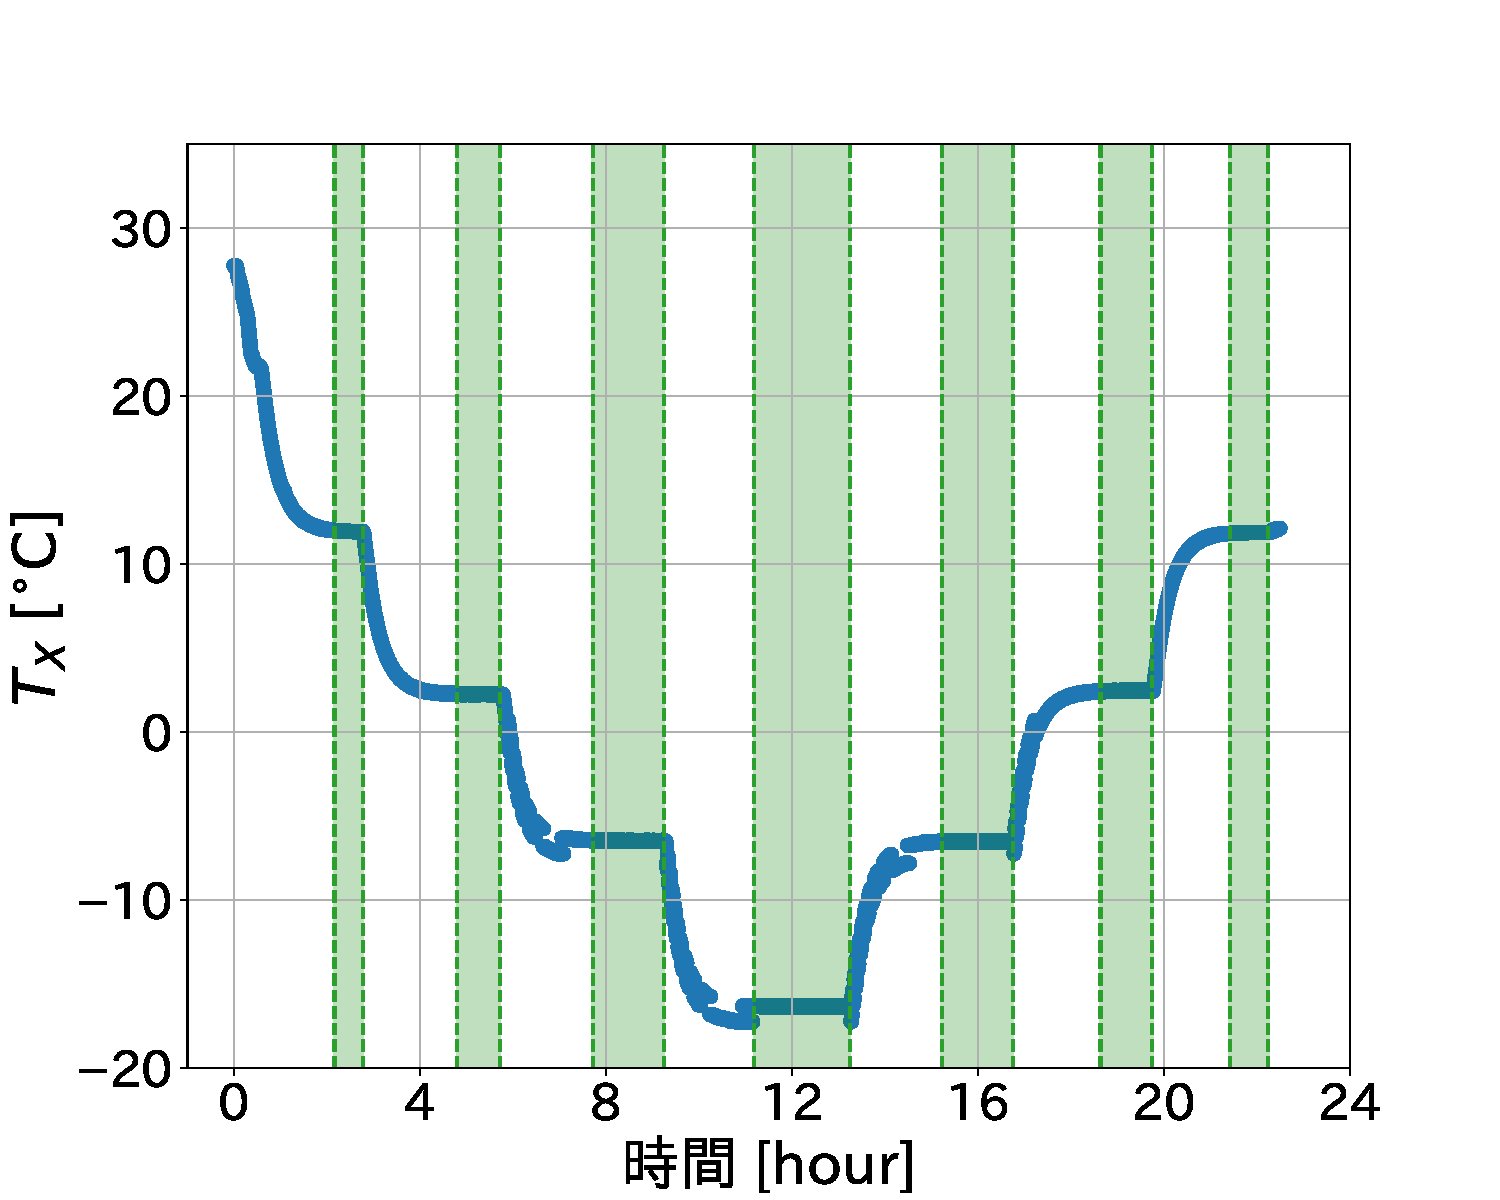
\includegraphics[width=1.1\columnwidth]{tiltsensor/bath_tempX.pdf}
        \subcaption{}
        \label{fig:bath_tempX}
    \end{minipage}
    \hspace{0.005\columnwidth}
    \begin{minipage}[b]{0.45\columnwidth}
        \centering
        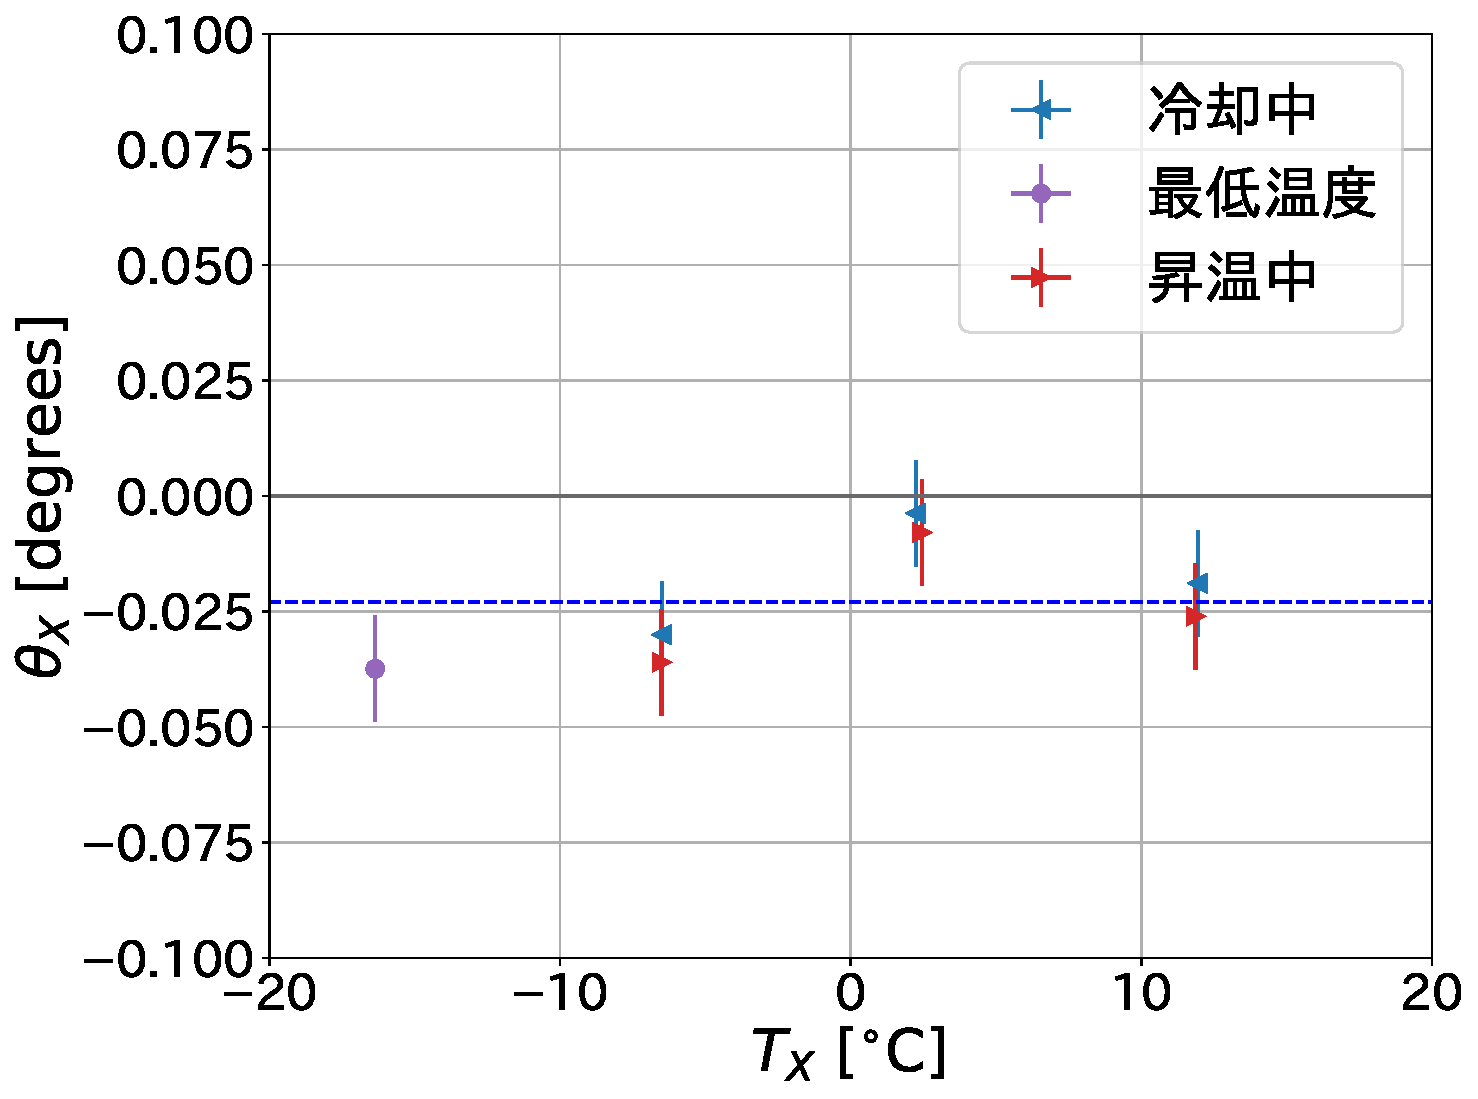
\includegraphics[width=1.065\columnwidth]{tiltsensor/angleX_temp_dep.pdf}
        \subcaption{}
        \label{fig:angleX_temp_dep}
    \end{minipage}
    \caption{重力参照計の $X$ 軸の温度変化と出力角度の変化。
             (\subref{fig:bath_tempX}) $X$ 軸の温度 $T_{X}$ の変化と切り取った温度安定区間。
             (\subref{fig:angleX_temp_dep}) $X$ 軸の出力角度 $\theta_{X}$ の温度依存性。}
    \label{fig:evaluation_bath_Xaxis}
\end{figure}
\begin{figure}[H]
    \begin{minipage}[b]{0.45\columnwidth}
        \centering
        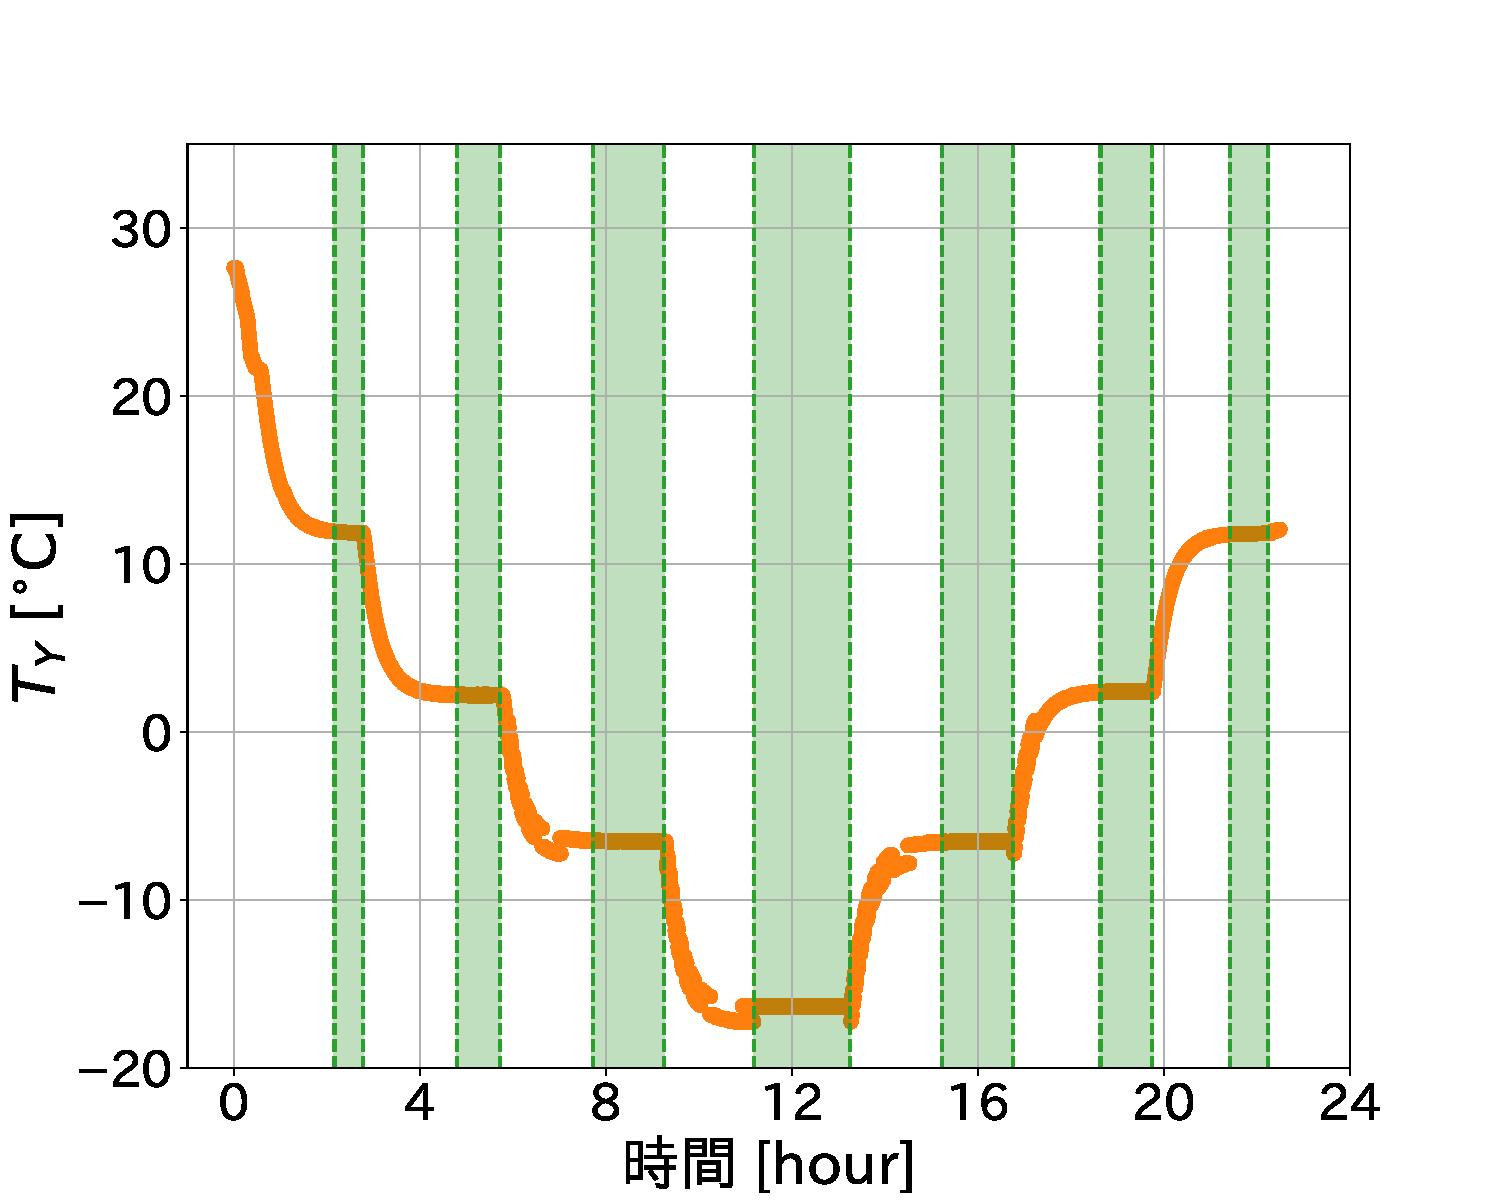
\includegraphics[width=1.1\columnwidth]{tiltsensor/bath_tempY.pdf}
        \subcaption{}
        \label{fig:bath_tempY}
    \end{minipage}
    \hspace{0.005\columnwidth}
    \begin{minipage}[b]{0.45\columnwidth}
        \centering
        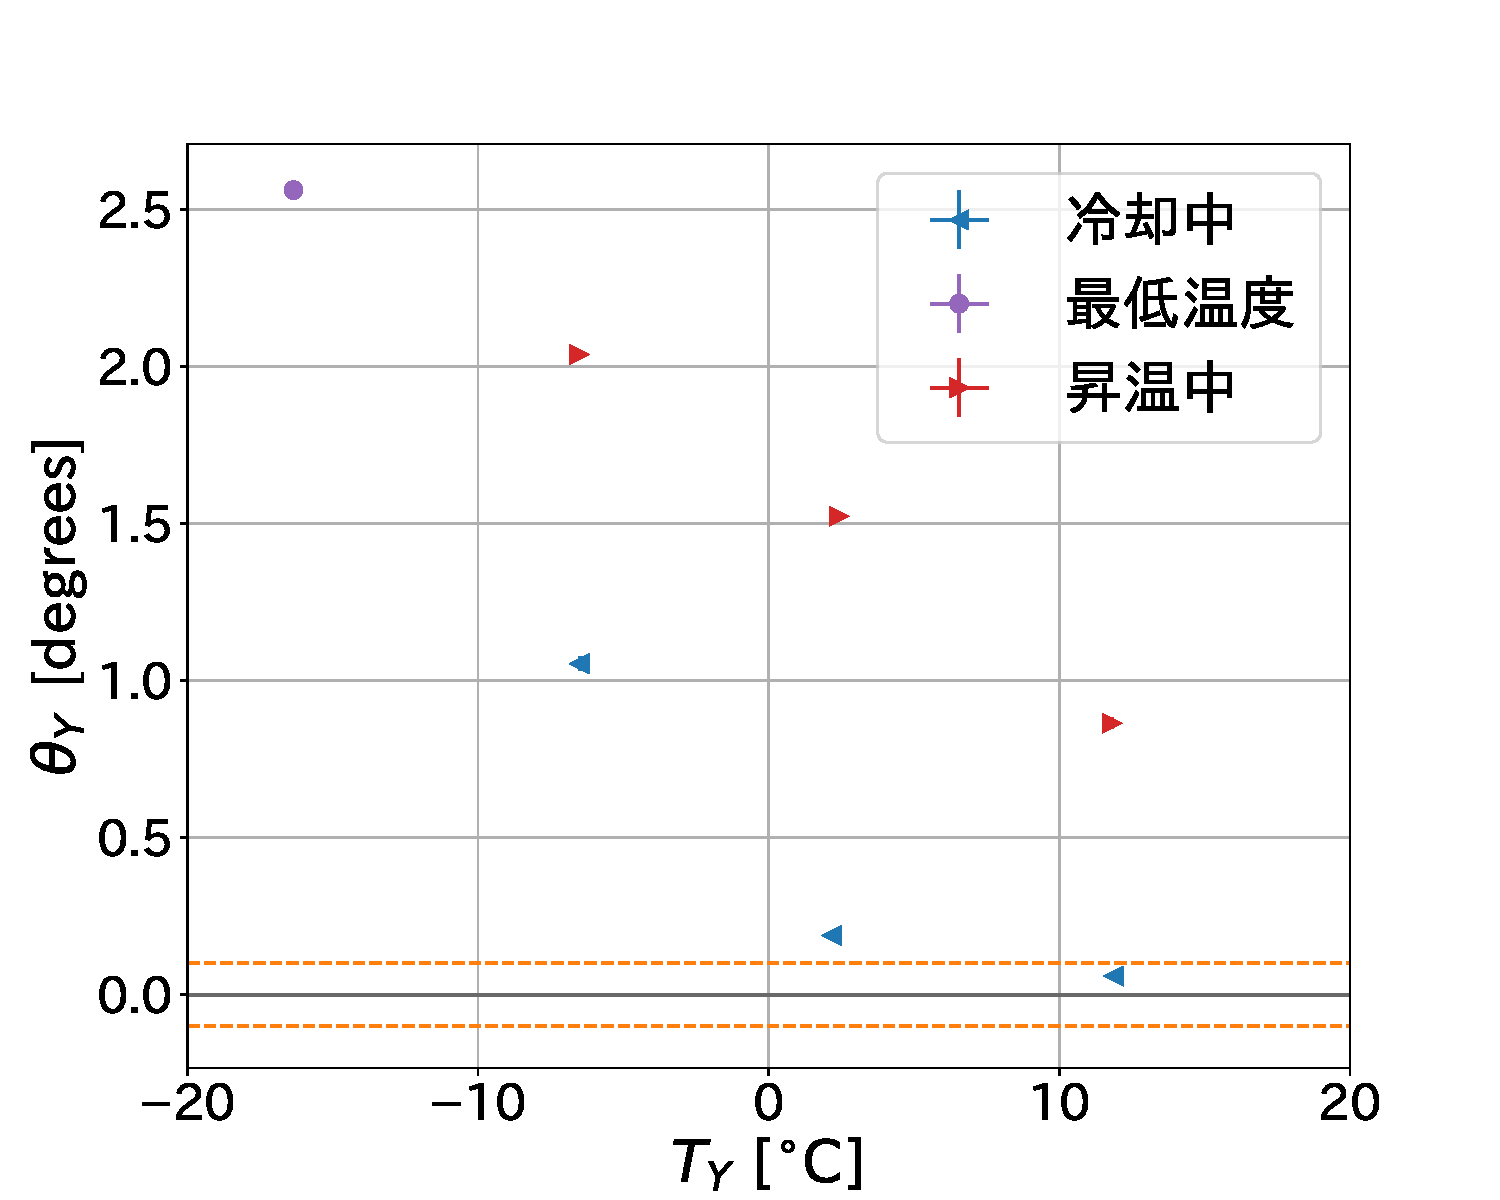
\includegraphics[width=1.03\columnwidth]{tiltsensor/angleY_temp_dep.pdf}
        \subcaption{}
        \label{fig:angleY_temp_dep}
    \end{minipage}
    \caption{重力参照計の $Y$ 軸の温度変化と出力角度の変化。
             (\subref{fig:bath_tempY}) $Y$ 軸の温度 $T_{Y}$ の変化と切り取った温度安定区間。
             (\subref{fig:angleY_temp_dep}) $Y$ 軸の出力角度 $\theta_{Y}$ の温度依存性。}
    \label{fig:evaluation_bath_Yaxis}
\end{figure}
\begin{table}[H]
    \centering
    \caption{温度変動による重力参照計の出力の変化の評価結果}
    \begin{tabular}{cccc} \hline
        & 平均 & 誤差の平均 & 精度 \\ \hline\hline
        $X$ 軸 & $-0.023\tcdegree$ & $0.011\tcdegree$ & $0.033\tcdegree$ \\ \hline
        $Y$ 軸 & $1.18\tcdegree$ & $0.014\tcdegree$ & $>1\tcdegree$ \\ \hline
    \end{tabular}
    \label{tab:temp_result}
\end{table}
\section{初期不良の検証}
\subsection{評価系}
前節にて行った温度変化に対する出力角度の評価にて判明した $Y$ 軸の出力角度の精度不良が初期不良によるものなのか、
それとも評価系の問題によるものなのかを検証するため、京都大学にていくつかの条件のもと評価を行った。
評価系を図\ref{fig:evaluation_system_kyoto}および図\ref{fig:evaluation_kyoto}に示す。
\begin{enumerate}
    \item[条件1.] 前節と同じ評価系を再現し、恒温槽に入れて温度変化に対する出力角度の変化を測定する。
                 (図\ref{fig:evaluation_kyoto}(\subref{fig:evaluation_kyoto1}))
    \item[条件2.] 条件1.の評価系において、アルミプレートごと系全体を $90\tcdegree$ 回転させ、温度変化に対する出力角度の変化を測定する。
                 これにより、恒温槽の床が温度変化により傾き、 $Y$ 軸の出力角度に影響を与えたのかを検証する。
                 (図\ref{fig:evaluation_kyoto}(\subref{fig:evaluation_kyoto2}))
    \item[条件3.] 条件2.の評価系において、重力参照計を $90\tcdegree$ 回転させ、再び温度変化に対する出力角度の変化を測定する。
                 これにより、アルミプレート自体が温度変化により傾き、それが $Y$ 軸の出力角度に影響を与えたのかを検証する。
                 (図\ref{fig:evaluation_kyoto}(\subref{fig:evaluation_kyoto3}))
\end{enumerate}
恒温槽は ETAC 社の HIFLEX FL211C を使用した。
温度変化は $\SI{30}{\degreeCelsius}$ から $\SI{-20}{\degreeCelsius}$ まで $90$ 分かけて冷却し、
恒温槽の温度と重力参照計の温度が安定するまで待った。その後再び $90$ 分ほどかけて $\SI{30}{\degreeCelsius}$ まで昇温した。
\begin{figure}[H]
    \centering
    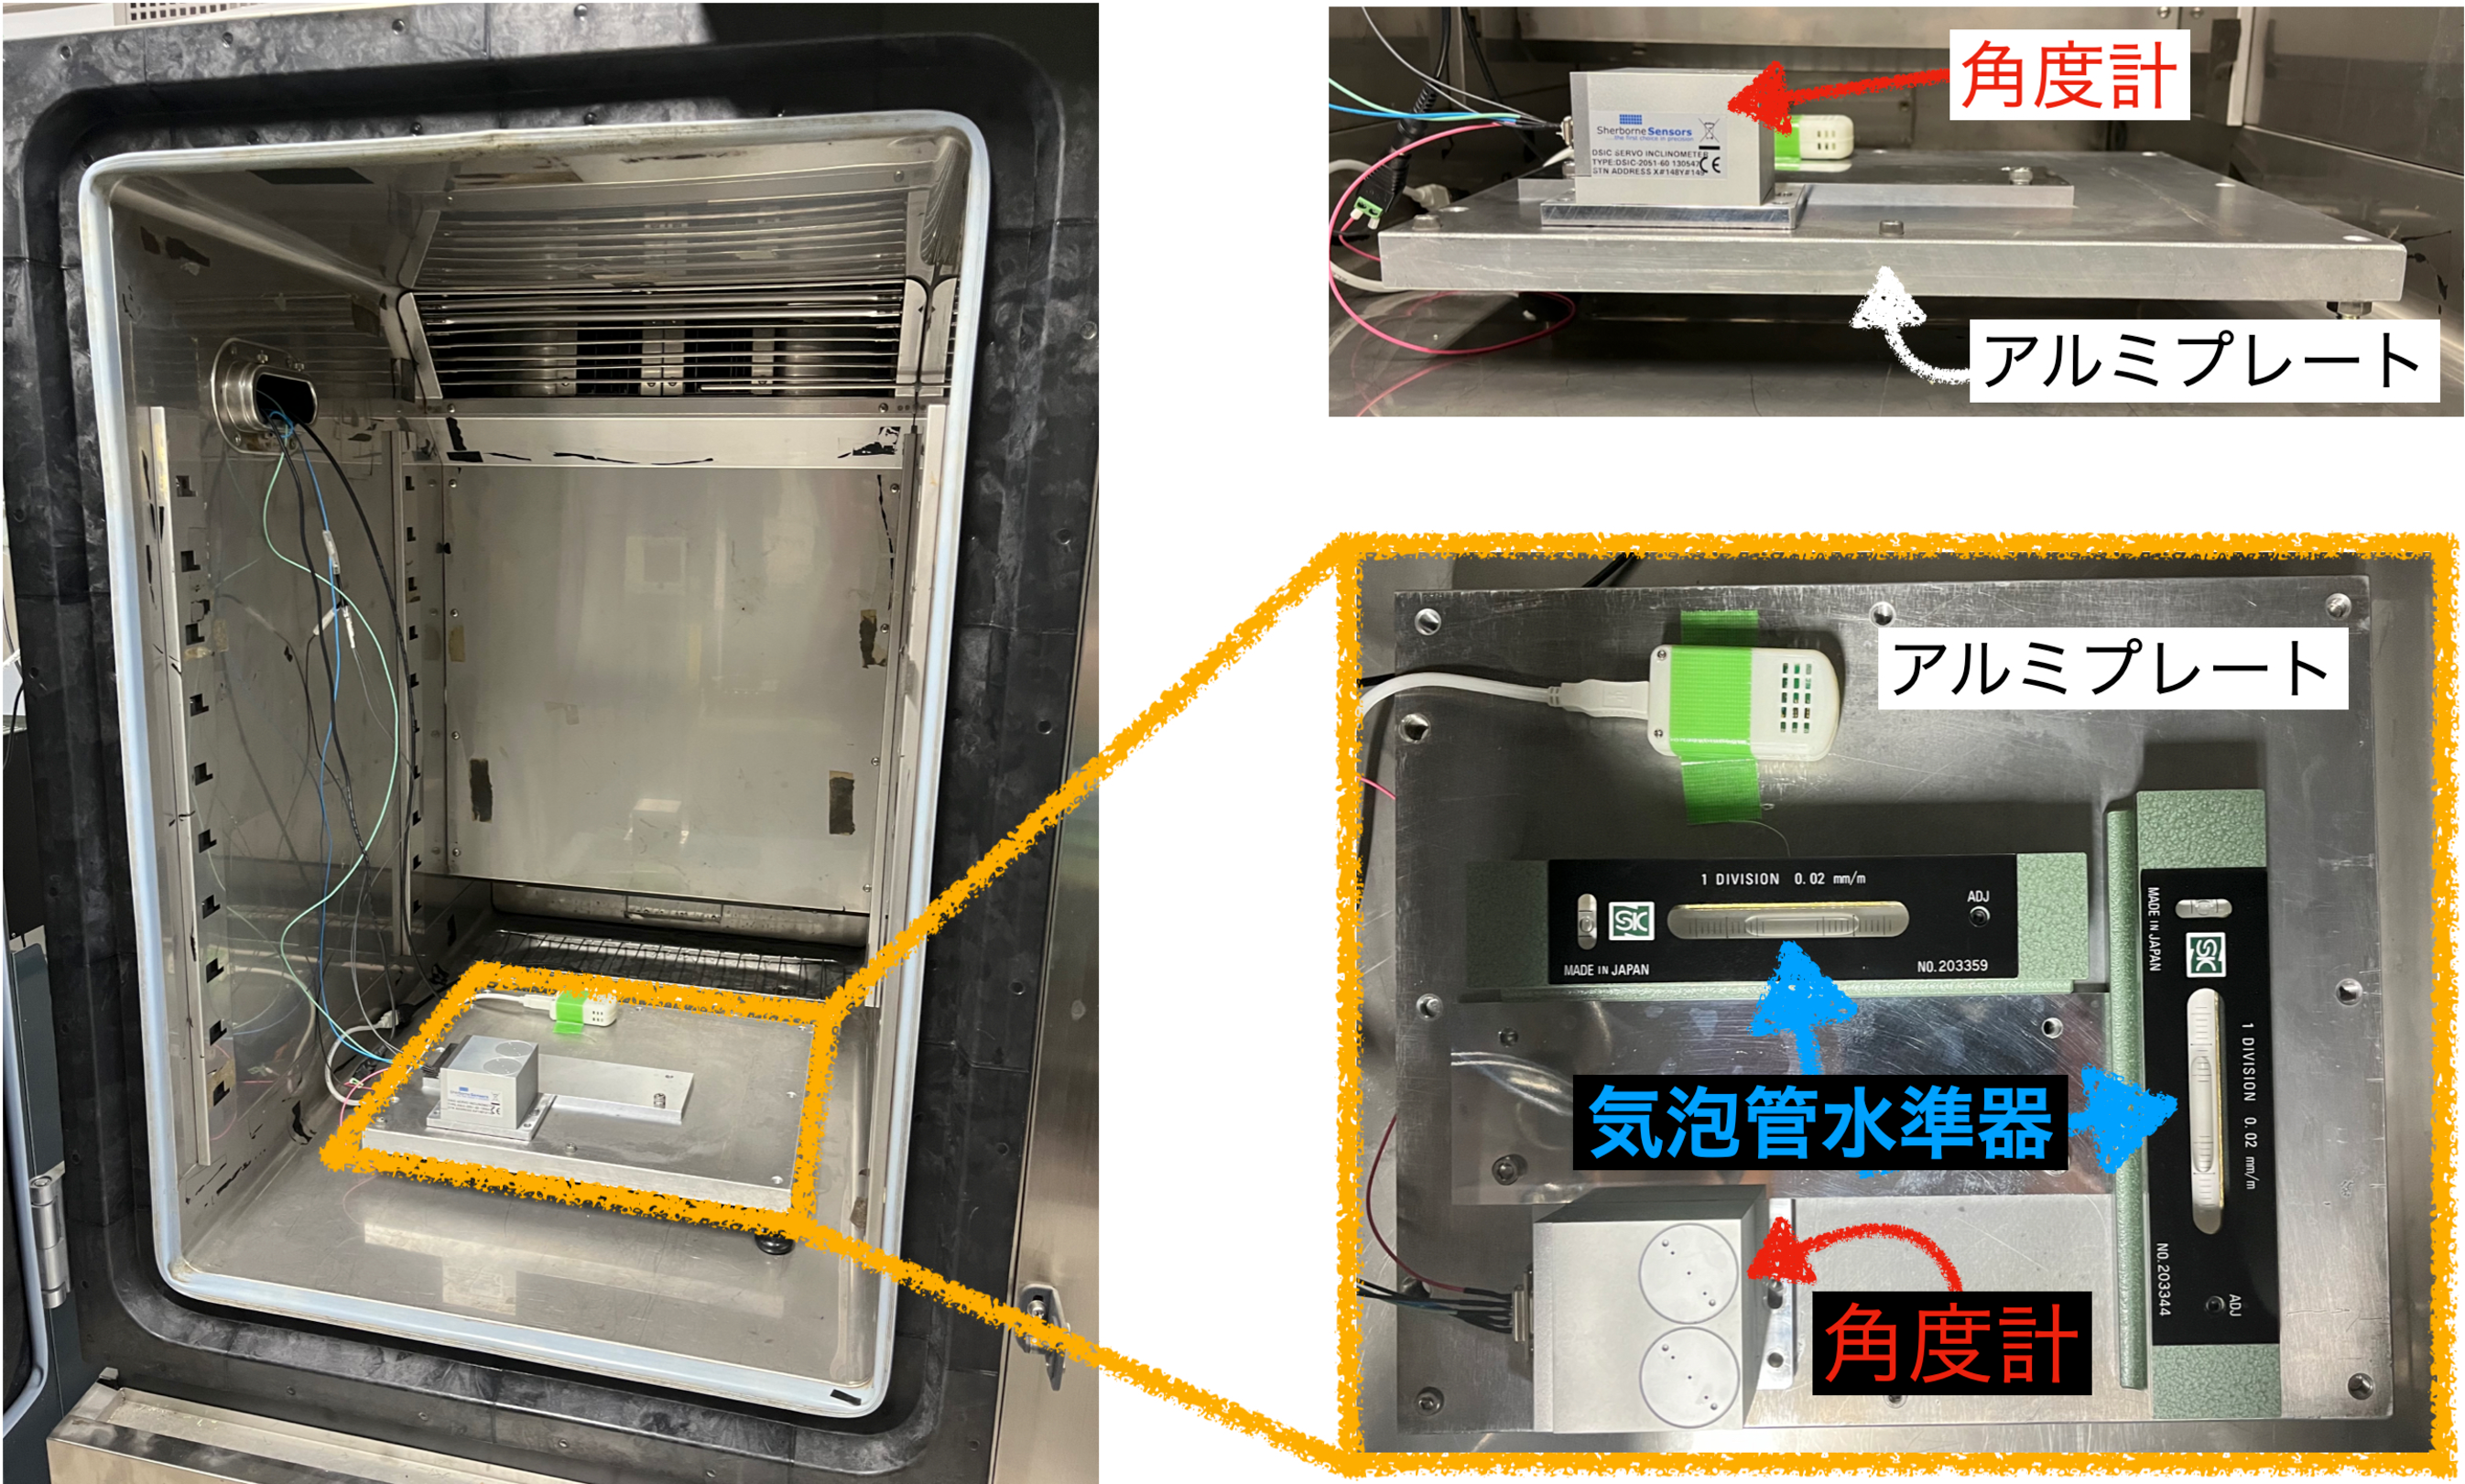
\includegraphics[width=0.75\textwidth]{tiltsensor/evaluation_system_kyoto.pdf}
    \figcaption{京都大学における重力参照計の初期不良検証系と恒温槽}
    \label{fig:evaluation_system_kyoto}
\end{figure}
\begin{figure}[H]
    \centering
    \begin{minipage}[b]{0.5\columnwidth}
        \centering
        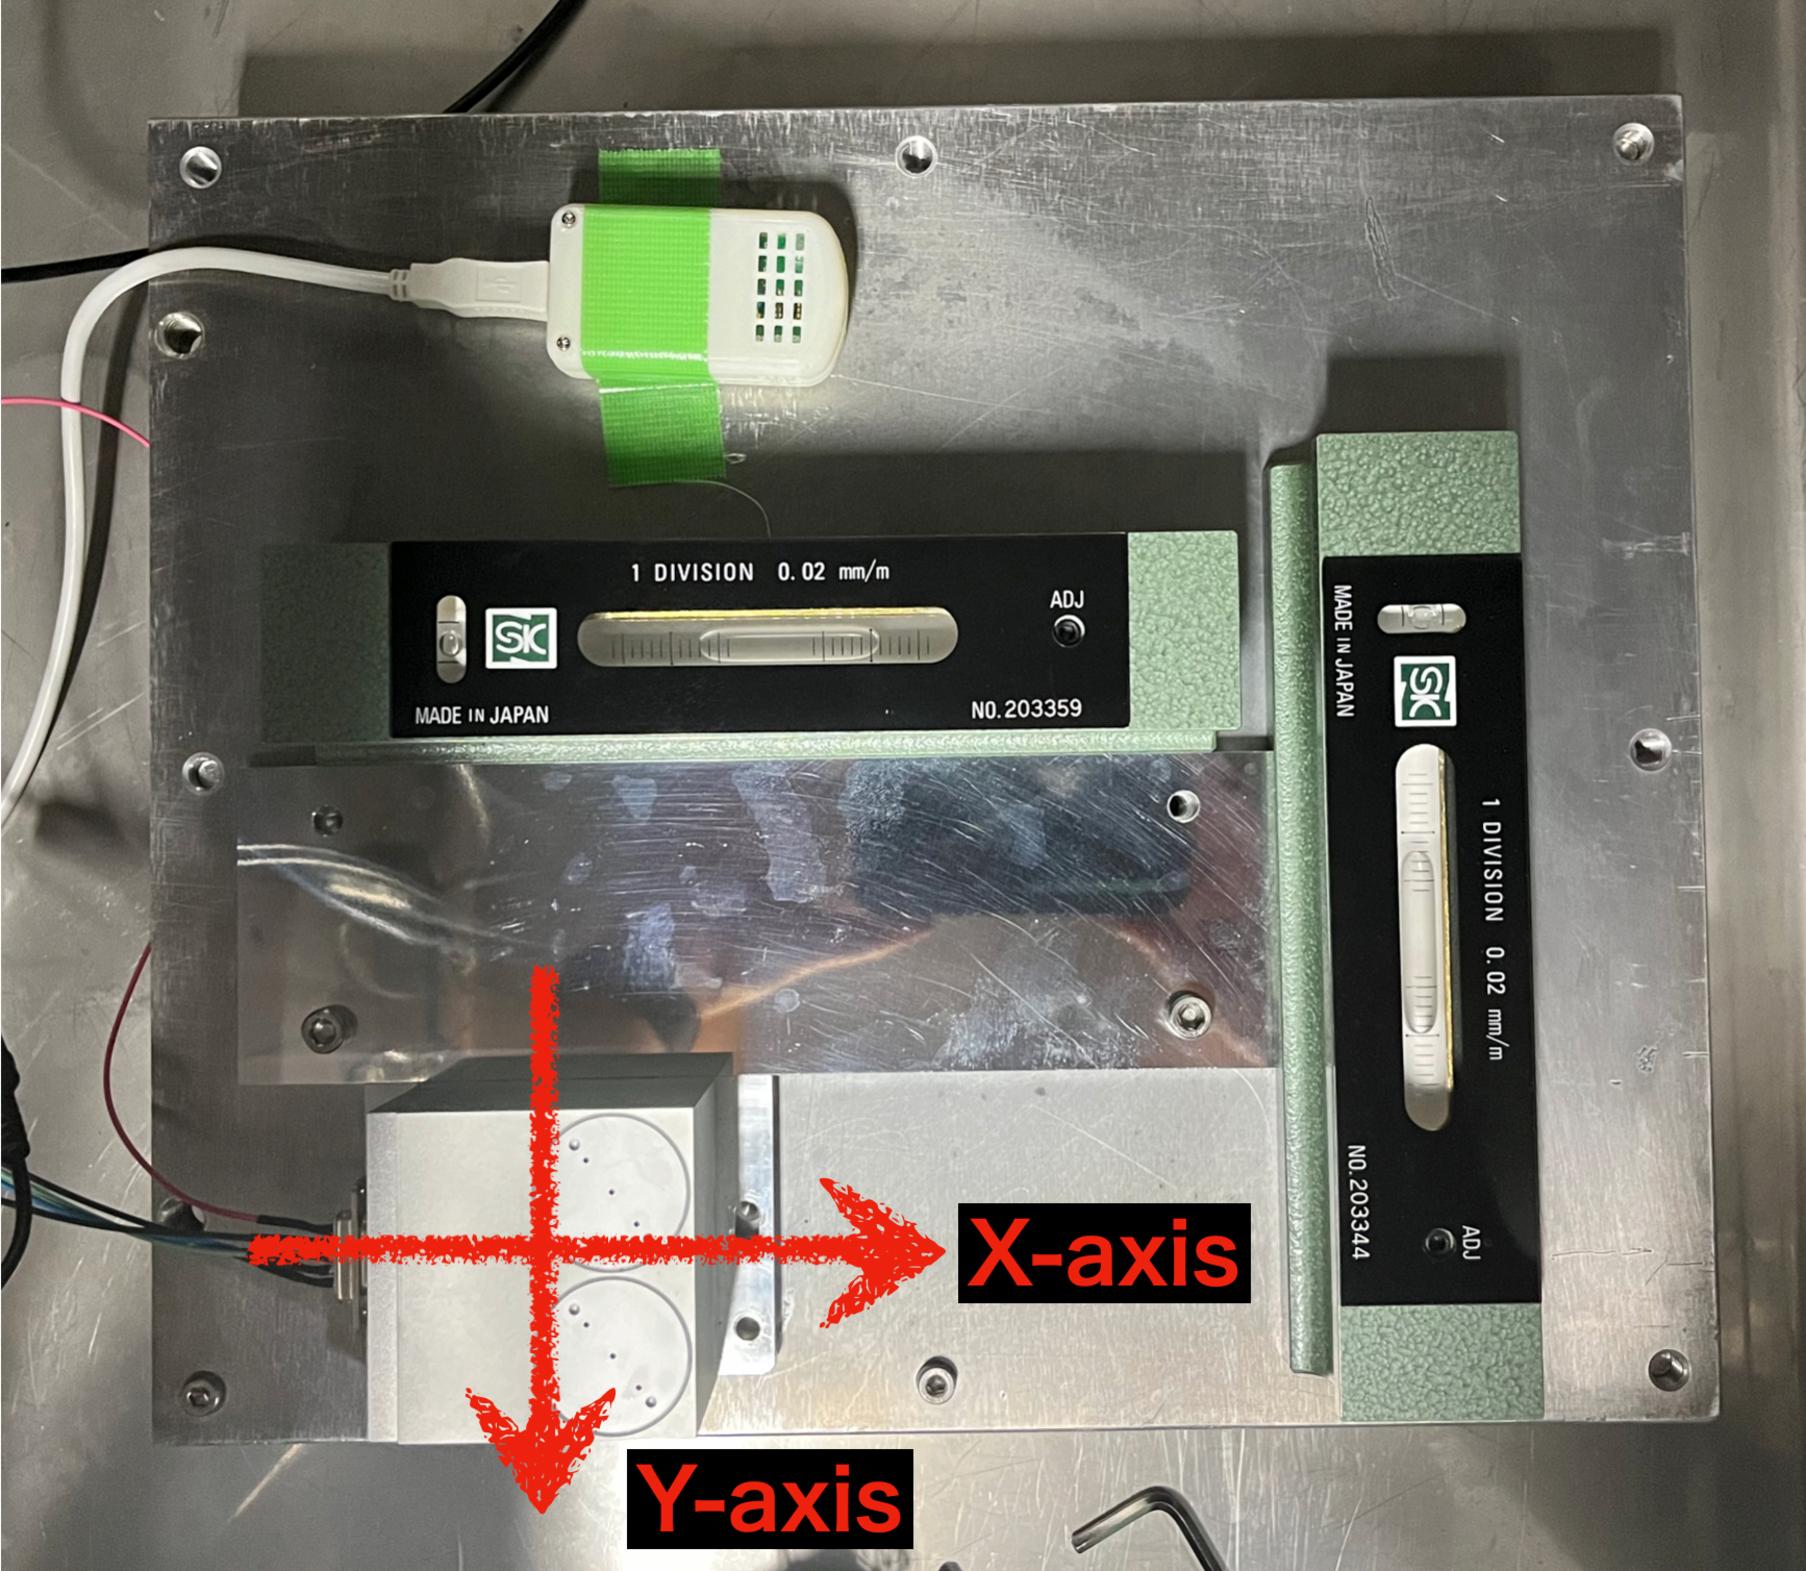
\includegraphics[width=0.9\textwidth]{tiltsensor/evalu_kyoto1.pdf}
        \subcaption{}
        \label{fig:evaluation_kyoto1}
    \end{minipage}
    %\hspace{0.005\columnwidth}
    \\
    \begin{minipage}[b]{0.42\columnwidth}
        \centering
        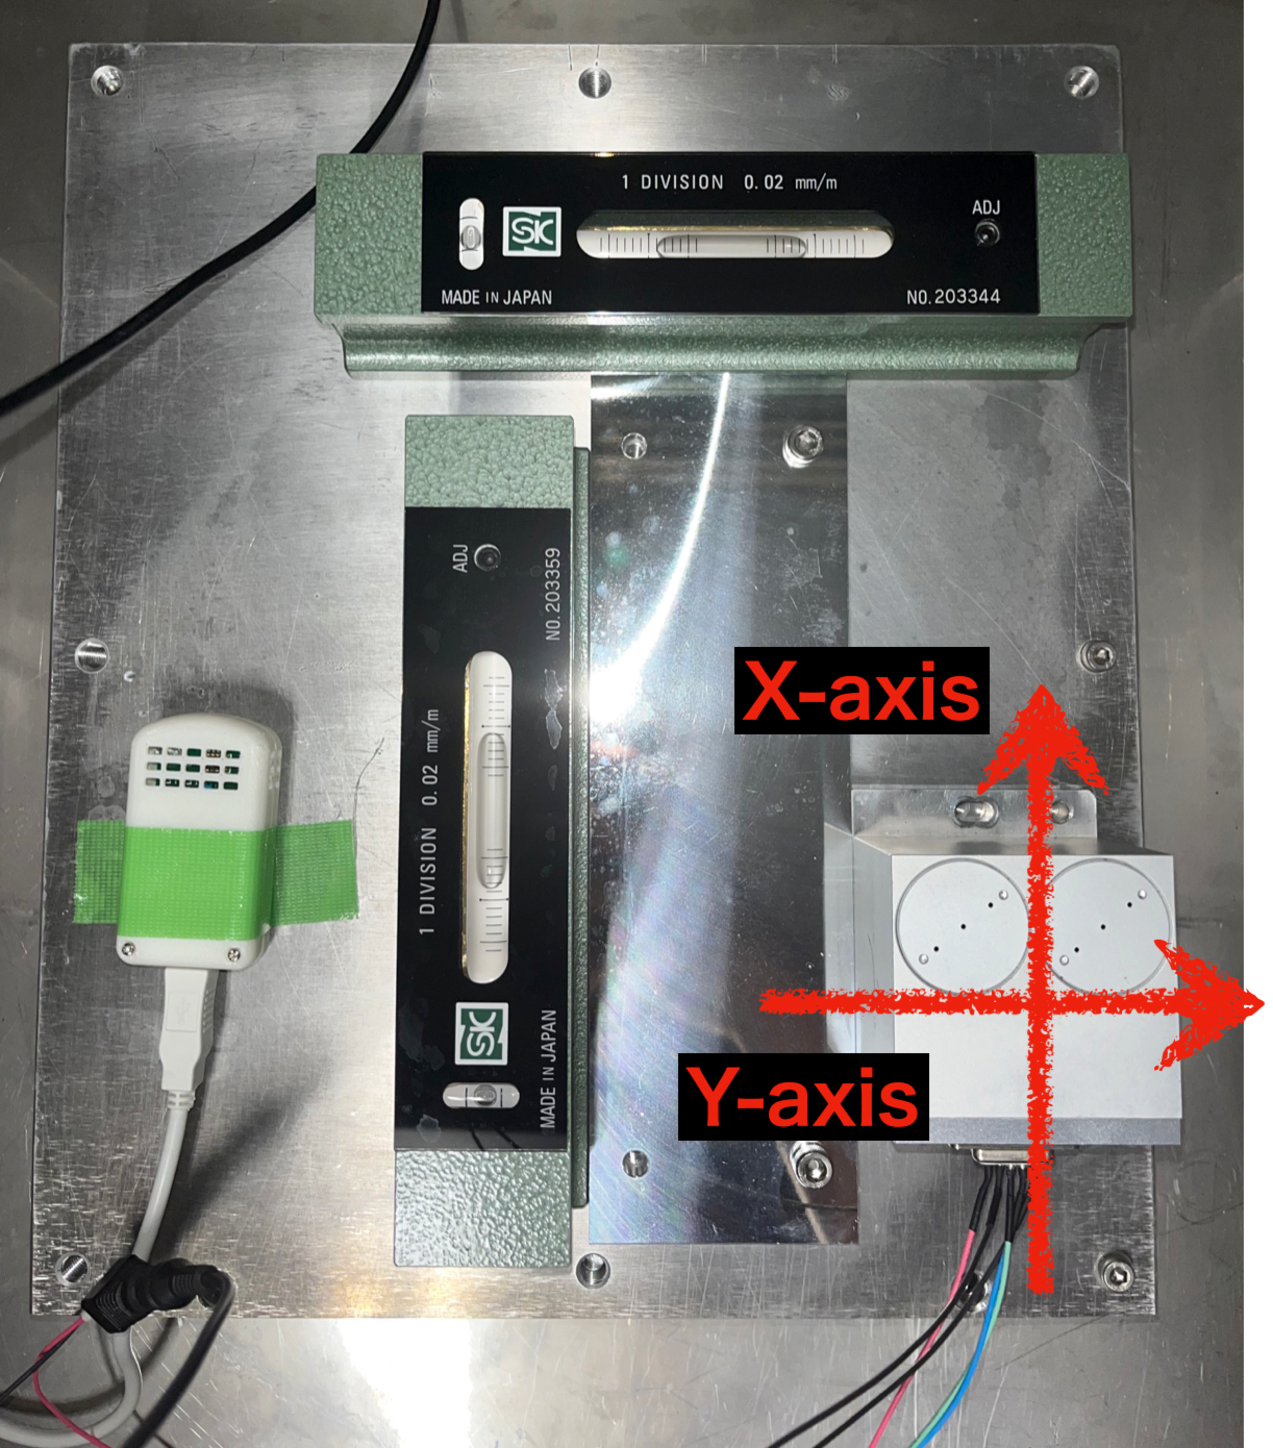
\includegraphics[width=0.8\textwidth]{tiltsensor/evalu_kyoto2.pdf}
        \subcaption{}
        \label{fig:evaluation_kyoto2}
    \end{minipage}
    %\hspace{0.005\columnwidth}
    \begin{minipage}[b]{0.455\columnwidth}
        \centering
        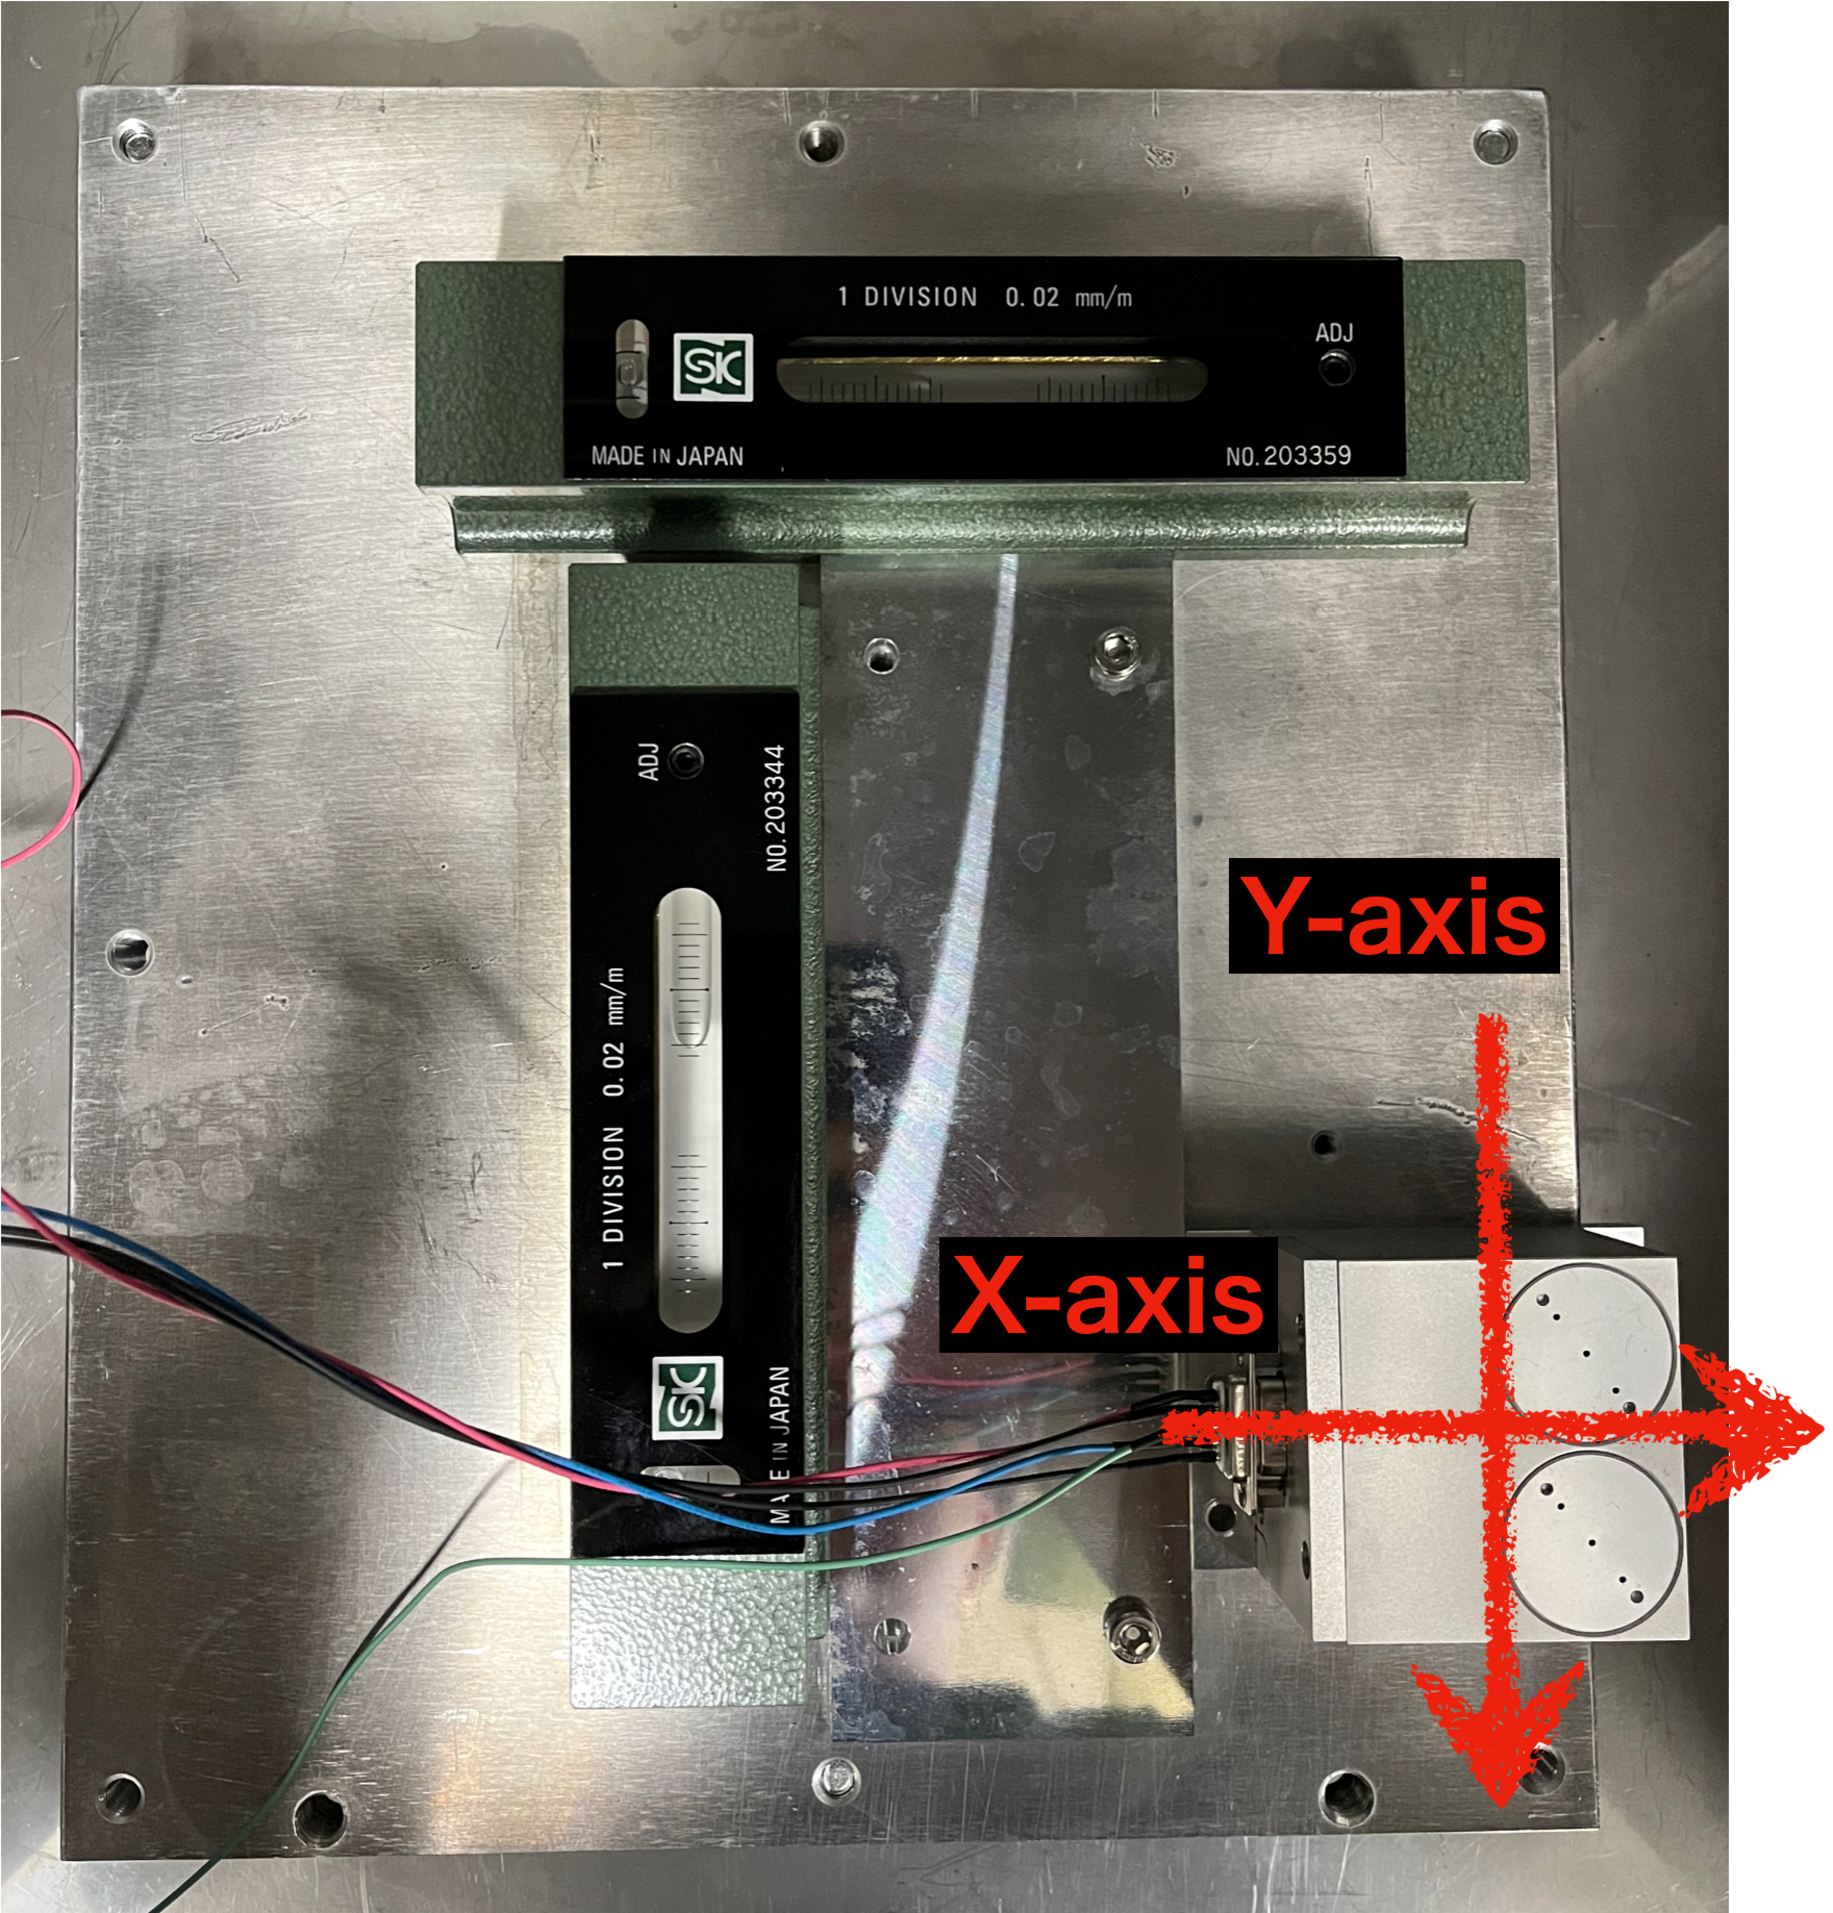
\includegraphics[width=0.8\textwidth]{tiltsensor/evalu_kyoto3.pdf}
        \subcaption{}
        \label{fig:evaluation_kyoto3}
    \end{minipage}
    \caption{各条件による重力参照計の初期不良検証系の違い。
             (\subref{fig:evaluation_kyoto1}) 条件1.の評価系。
             (\subref{fig:evaluation_kyoto2}) 条件2.の評価系。
             (\subref{fig:evaluation_kyoto3}) 条件3.の評価系。}
    \label{fig:evaluation_kyoto}
\end{figure}
\subsection{評価結果とその考察}
図\ref{fig:angleY_huryou_test}に、各条件$1\sim3$での温度変化に対する $Y$ 軸の出力角度の変化を示す。
いずれの条件においても、公称精度である $0.08\tcdegree$ を大きく上回る出力角度の変化が見られた。
また、その傾向はいずれの条件においても一致しており、恒温槽の床の変形やアルミプレートの変形が原因ではないと結論づけられる。
以上の検証をもとに本重力参照計は初期不良があると判断し、メーカーによる修理を依頼した。
修理が終了し次第、$Y$ 軸の精度を再評価する必要がある。

なお、氷点下の温度において測定値のばらつきが生じているが、本測定では90分で$\SI{50}{\degreeCelsius}$近く温度を上げ下げする急激な温度変化を行っており、
重力参照計の温度が安定しているときにはこのようなばらつきは見られなかったため、このばらつきは温度の急激な変化によるものだとみなすことができる。
観測サイトではこのような急激な温度変化は生じないため、偏光角較正装置に搭載する際には問題ないと考えられる。
\begin{figure}[H]
    \centering
    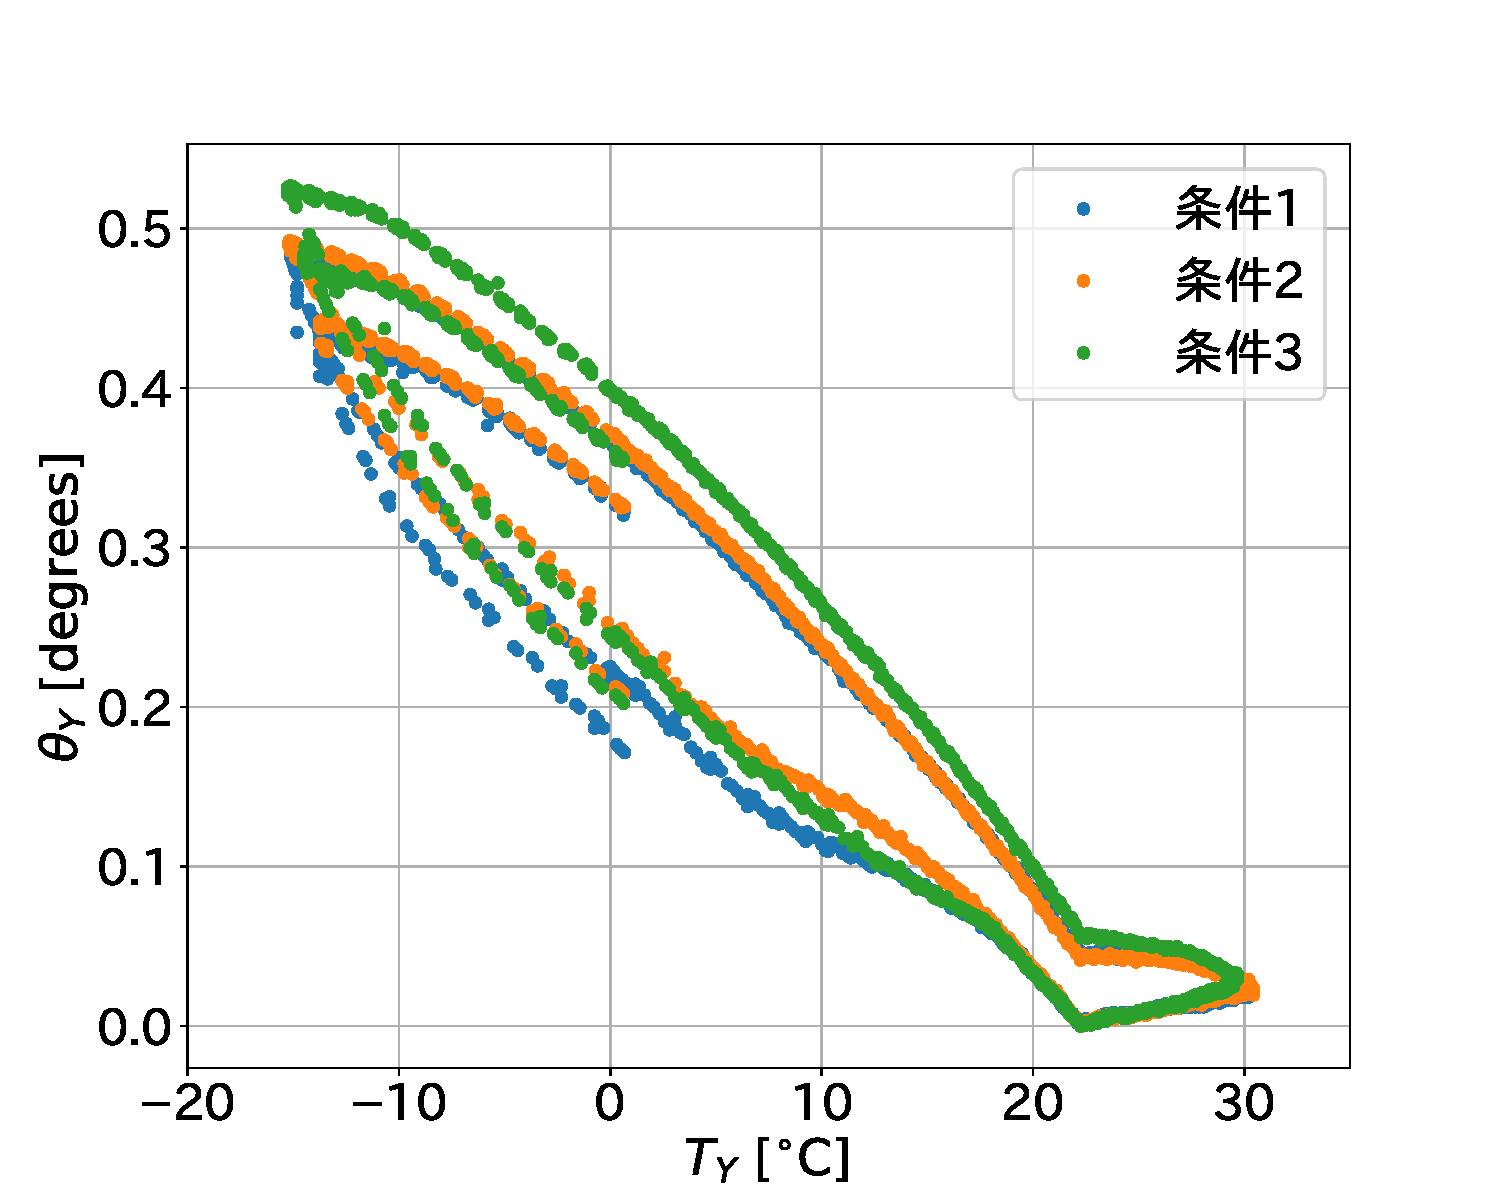
\includegraphics[width=0.8\textwidth]{tiltsensor/angleY_huryou_test.pdf}
    \figcaption{各条件における $Y$ 軸の出力角度の温度変化}
    \label{fig:angleY_huryou_test}
\end{figure}

\section{まとめと$\theta_{\mathrm{ses}}$の誤差}
本章では、重力参照計 Sherborne Sensors 社 DSIC-2051-60 の評価を行った。
長期間の実験期間にて絶対角度の精度を保証するため、長期間の出力の安定性を評価した。
また、観測サイトの気温の変化に耐えうるかを確認するため、恒温槽を用いて温度変化に対する出力角度の変化を測定した。
長期安定性に関しては、 $X$ 軸の精度が $\delta\theta_{X,\mathrm{time}} = 0.003\tcdegree$ であり、
$Y$ 軸の精度が $\delta\theta_{Y,\mathrm{time}} = 0.034\tcdegree$ と評価された。
温度変化に対する出力角度の変化に関しては、 $X$ 軸の精度が $\delta\theta_{X,\mathrm{temp}} = 0.033\tcdegree$ であり、
$Y$ 軸の精度が $\delta\theta_{Y,\mathrm{temp}} > 1\tcdegree$ と評価された。
この結果から、 $\theta_{X}$ の精度を 
\begin{equation}
    \delta\theta_X = \sqrt{\qty(\delta\theta_{X,\mathrm{time}})^2 + \qty(\delta\theta_{X,\mathrm{temp}})^2}\simeq 0.033\tcdegree < 0.04\tcdegree
\end{equation}
であると結論づけた。これは要求精度を満たすものである。
$Y$ 軸に関しては、公称精度を大きく上回る $2.0\tcdegree$ 以上の出力角度の変化が見られ、初期不良の可能性が疑われた。
その後の検証を経て、初期不良であることが確認され、メーカーによる修理を依頼した。

$Y$ 軸は初期不良により要求を満たさなかったが、修理により $X$ 軸と同程度の精度を達成できると期待される。
すなわち、本重力参照計の各軸の精度は $\delta\theta_X\sim\delta\theta_Y<0.04\tcdegree$ となり、要求精度を満たすと見込んでいる。

実際に望遠鏡の偏光角較正の精度として
\end{document}